The reference-predication trade-off hypothesis was tested in four preregistered behavioural web-based experiments employing different dependent measures. The crucial manipulation in all experiments was the varying position of the critical noun - it appeared either in the subject (e.g., “That N is ADJ” or “That ADJ N is N2”) or in the predicate (“That’s a ADJ N” or “That N2 is a ADJ N”) of the sentences presented in the experiments. These sentences described a depicted object which appeared in visual context. 

These objects were sampled from five different \textit{basic-level} categories: dogs, birds, flowers, trees and fish \parencite{rosch1976}. Within each basic-level category, at least two \textit{subordinate} categories were chosen which exhibit a rather high or rather low amount of the feature described by the gradable adjectives under investigation - that is, those subordinate categories which people expect to be rather large or rather small representatives of their basic-level categories (s. Table \ref{tab:stimuli}). For example, for the \textit{dog}-category, the large-subordinate category \textit{Great Danes} and the small-subordinate category \textit{pugs} were chosen. As shown by \textcite{tessler2017warm}, when encountering representatives of such categories described by the adjective consistent with participants’ prior expectations about the degree of feature-under-discussion, people are a priori more likely to infer the basic-level comparison class than the subordinate comparison class. For example, when encountering the sentence “It’s big” said of a Great Dane (a large-subordinate category for the basic-level category dogs), humans are more likely to infer that the Great Dane is big relative to other dogs in general, than big relative to other Great Danes.  
Following the design of \textcite{tessler2017warm} in these experiments allows to test the effect of syntactic position of the noun on how strong the noun is taken to constrain the comparison class: The reference-predication trade-off hypothesis predicts that nouns in the predicate position constrain the comparison class more strongly than in the subject position, such that a priori using the basic-level noun in predicate position is more felicitous in order to describe a normal-sized large-subordinate object (e.g., a Great Dane) than using a subordinate-label of the object in predicate position. Both nouns would be felicitous in the subject position. Furthermore, encountering a subordinate label in the predicate position, should signal a more extreme feature value than the basic-level label.

\begin{table}[t]
	\small{
		\begin{center}
			\caption{Experimental items: each basic-level context had two potential targets from an either saliently small or saliently big subordinate category within the basic-level class. Items marked with * were used only in Expt. 2., items marked with $^{+}$ were used in all experiments including Expt. 4}
			\label{tab:stimuli}
			\vskip 0.12in
			\fontsize{10}{11}\selectfont
			\begin{tabularx}{\textwidth}{XXX}
				\hline
				Basic-level category & Smaller referent & Bigger referent\\
				\hline
				Dogs$^+$ & Pug$^+$ & Great Dane$^+$ \\
				Dogs$^+$ & Chihuahua$^+$ & Doberman$^+$\\
				Birds$^+$ & Hummingbird$^+$ & Eagle$^+$  \\
				Fish & Goldfish & Swordfish \\
				Flowers$^+$ & Dandelion$^+$ & Sunflower$^+$\\
				Trees$^+$ & Bonsai$^+$ & Redwood$^+$\\
				Birds* & Sparrow* & Goose* \\
				Birds* & Canary* & Swan* \\
				Fish* & Clownfish* & Tuna* \\
				Flowers* & Daisy* & Peony* \\
				\hline     
			\end{tabularx}
		\end{center}
	}
\end{table}

Therefore, in all experiments, the referents were described by the adjective matching prior feature-degree expectations; for instance, Great Danes and sunflowers were always described as \textit{big}, and pugs or daisies as \textit{small}. 

\begin{figure*}[t]
	\begin{center}
		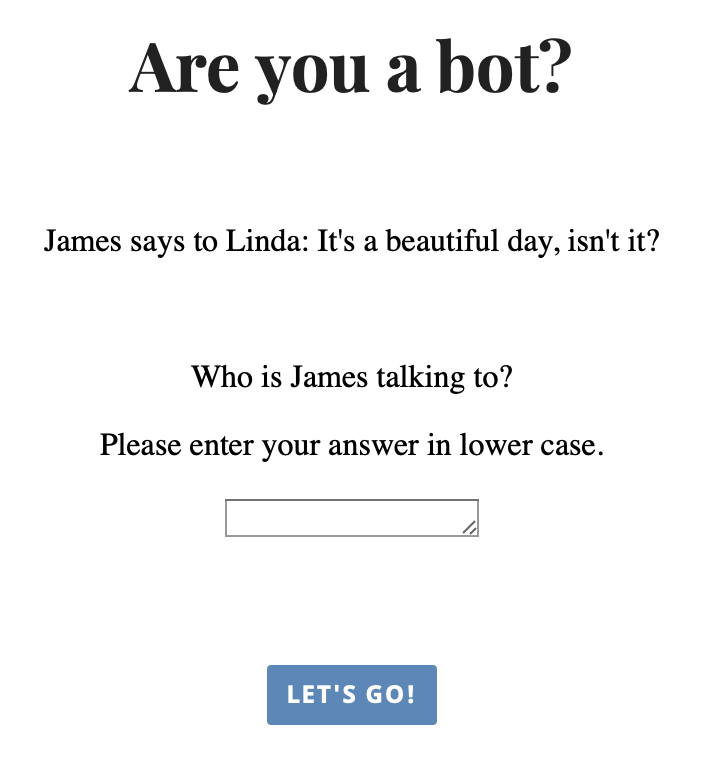
\includegraphics[width=0.5\linewidth]{captcha.png}
	\end{center}
	\caption{Example view of the bot check trial: The speaker James addresses the listener Linda.}
	\label{captcha}
\end{figure*}

The structure of all experiments was similar. First, participants completed a bot-check trial (Fig.~\ref{captcha}): Participants read a sentence where a named speaker asked a named listener: “It’s a beautiful day, isn’t it?”. The speaker and listener names were sampled from lists of ten popular male and female English names (s. Appendix \ref{appendix}). For example, the sentences read: “James says to Linda: 'It’s a beautiful day, isn’t?'; Who is James talking to?”.  Participants were asked to fill-in in lowercase who the listener is talking to. Participants were provided feedback and had maximally three attempts to fill-in the correct name. They were only allowed to proceed, if they successfully completed the bot check. Then, participants read instructions and completed practice trials, before completing main trials. After the main trials, they completed a socio-demographic post-test questionnaire, where they were asked to indicate their native language and optionally provide further information. 
For all experiments, participants were recruited via the crowd-sourcing platform Amazon’s Mechanical Turk; only participants with IP addresses in the United States and work approval rating of at least 95\% were permitted to participate. Participants were restrained from taking part in multiple experiments of this series.  

The first experiment (E1, Sentence Rating Experiment) was a sentence rating experiment, wherein participants had to rate two sentences which differed in the position of the noun (subject-N ~vs.~ predicate N) and the specificity of the noun (basic-level~vs.~subordinate label), as describing an object in context. 
In the second experiment (E2, Noun Production Experiment), participants had to fill-in the missing noun of a sentence describing the size of a referent in context. The position of the missing noun was varied. 
In the third experiment (E3, Comparison Class Inference Experiment), participants provided the inferred comparison classes via a free-production paraphrase, given sentences which varied by the noun category and its position, as describing a referent in different contexts. 
Finally, the fourth experiment (E4, Direct Modification Experiment) gathered inferred comparison classes in a paradigm akin to E3, but from sentences wherein the critical subordinate noun appearing in subject or predicate position was always syntactically modified by the adjective. 
All experimental materials and data can be found under \texttt{https://github.com/polina-tsvilodub/refpred}. All experiments were realized using the \_magpie - framework \parencite{magpie}. 
All experiments and preregistrations can be viewed under \texttt{tinyurl.com/yb5ogj5g}. \pt{preliminary link}

\section{Experiment 1: Sentence Rating Experiment}

%Results: main, by-participant / by-item variation, different exclusion criteria 

The aim of the sentence rating experiment was to investigate whether participants prefer one syntactic frame over the other, given two truth-conditionally equivalent sentences, depending on the noun category. The type of the noun and its syntactic position differed within-subjects.

\begin{figure*}[t]
	\begin{center}
	%	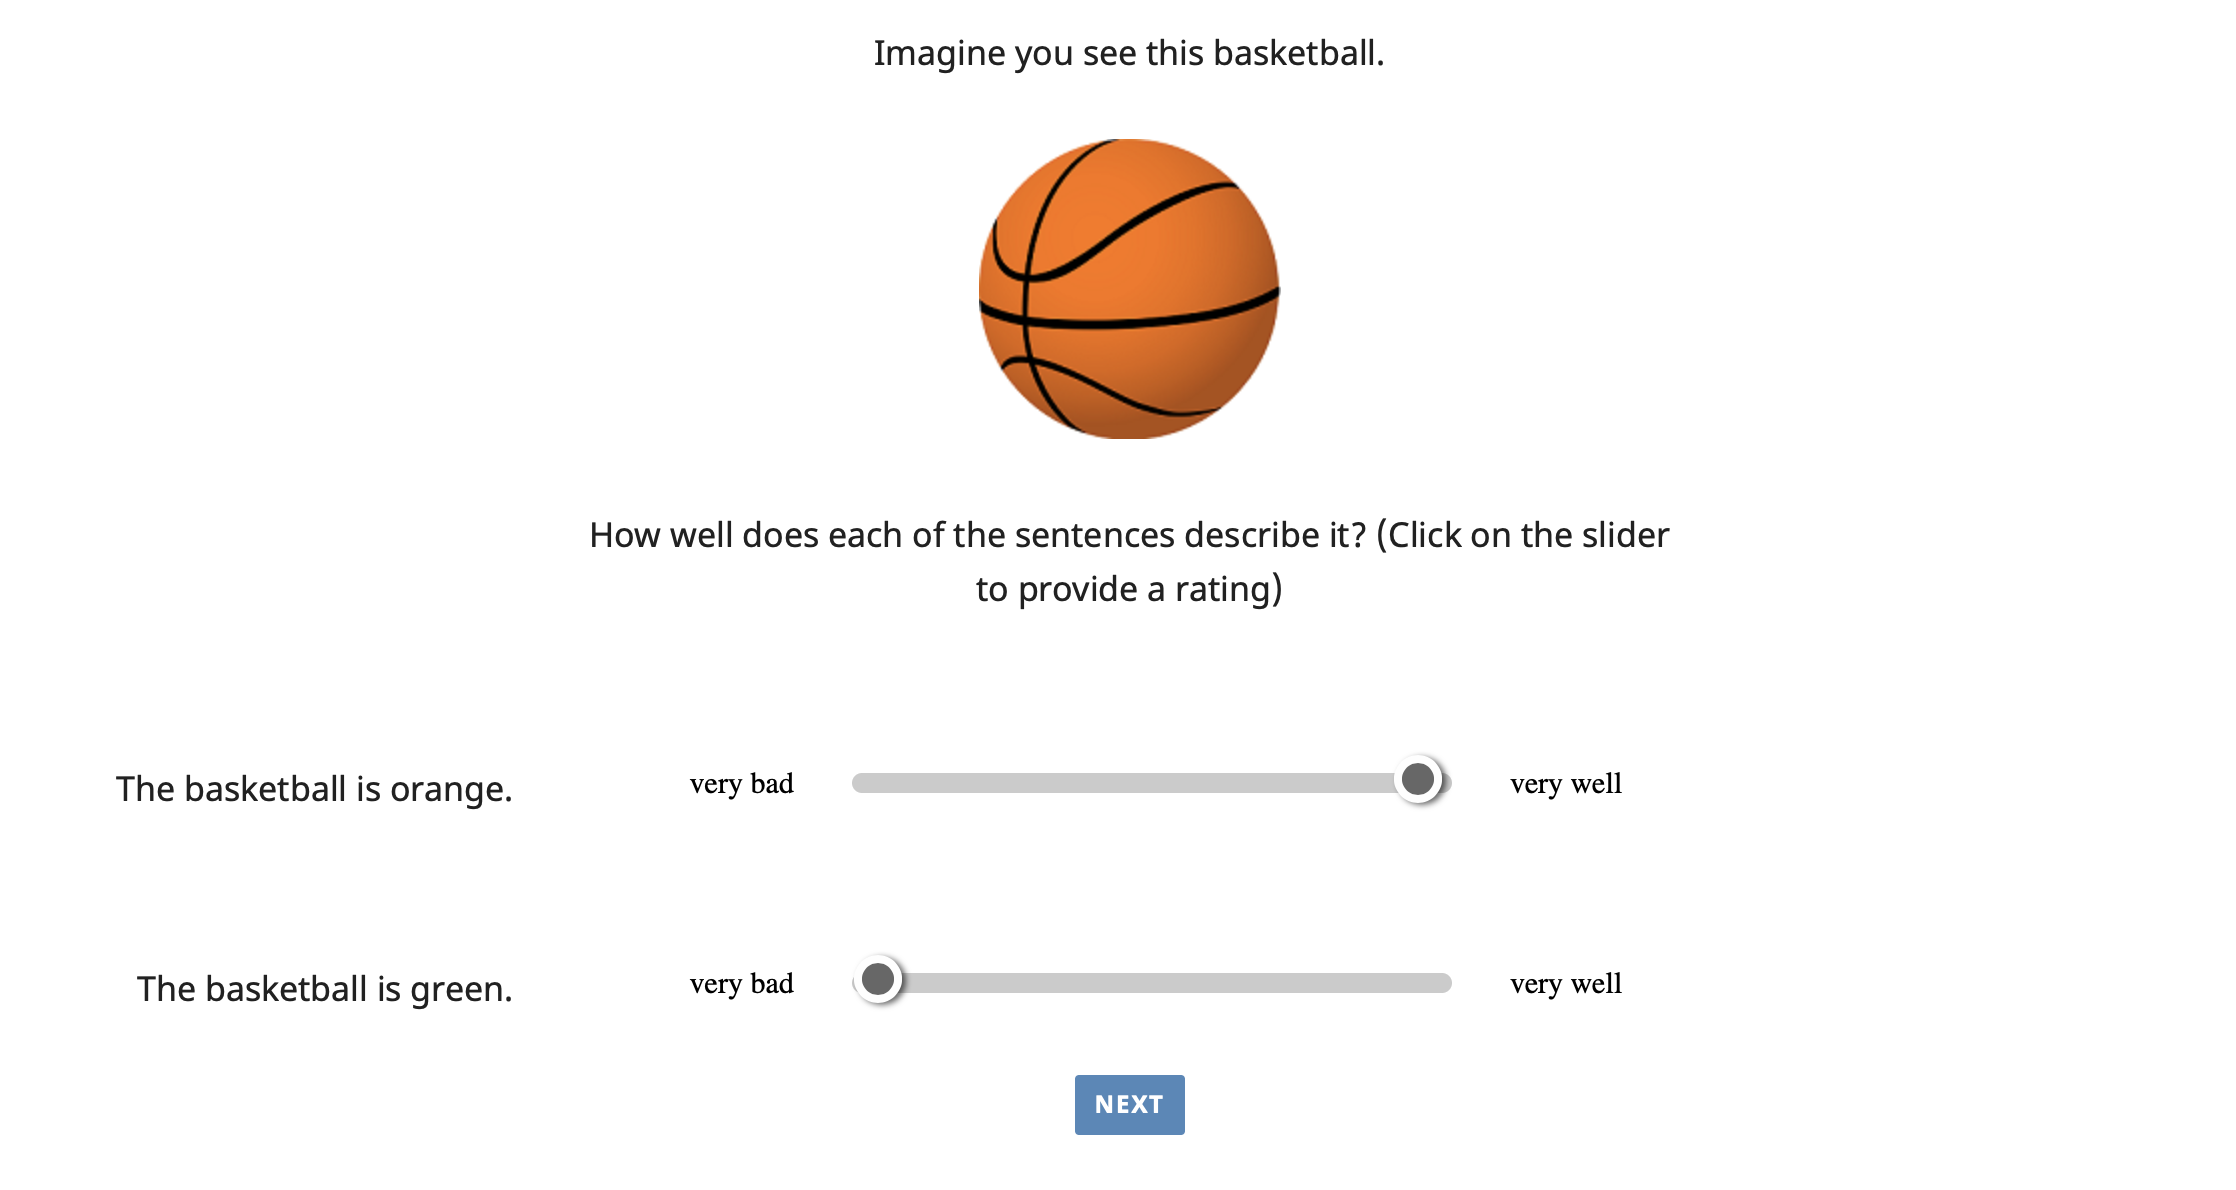
\includegraphics[width=0.7\linewidth]{warmup_basketball.png}
		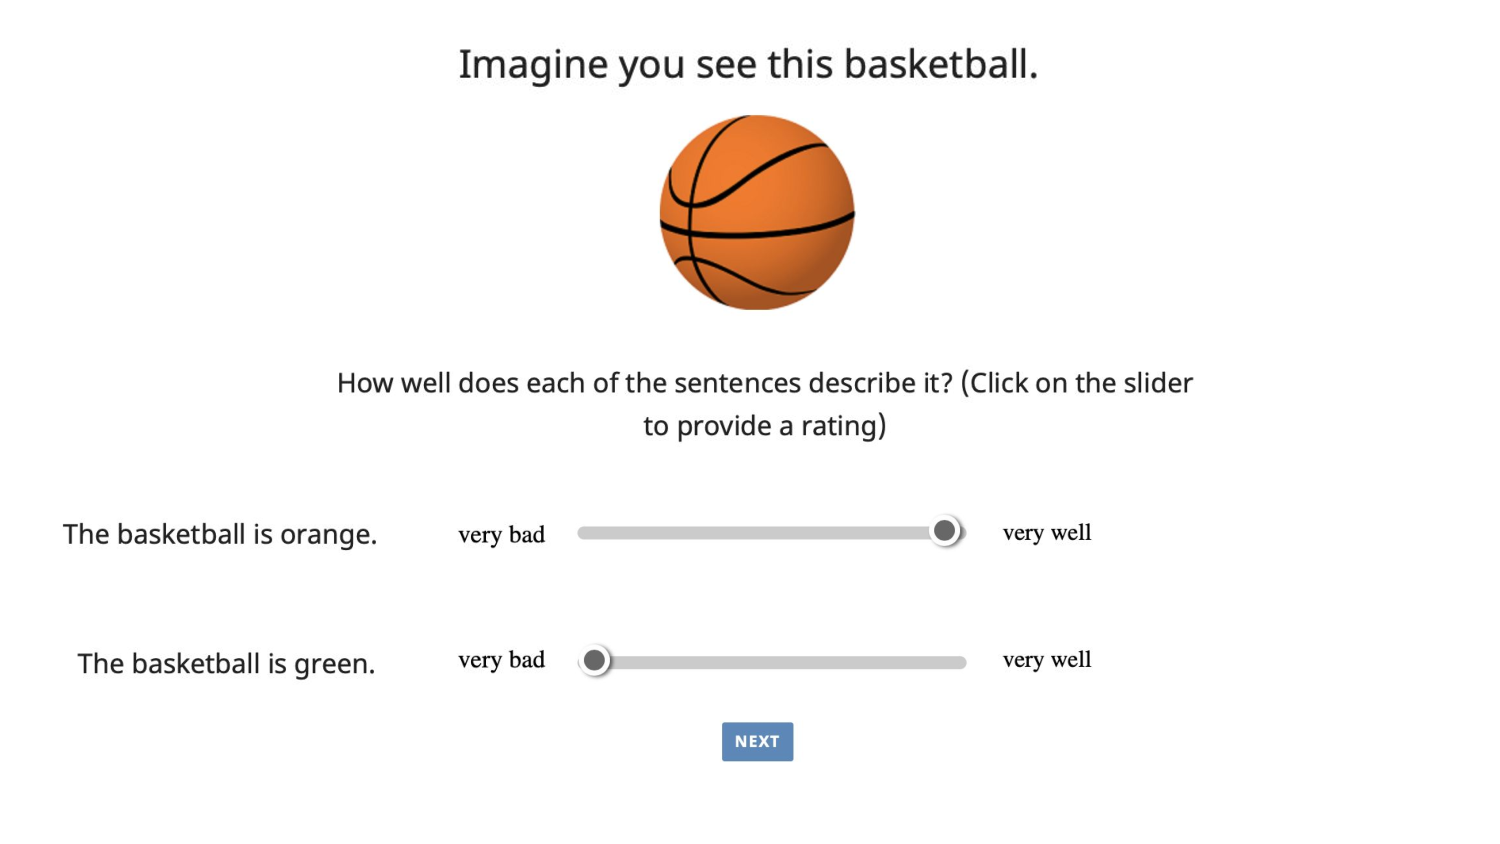
\includegraphics[width=0.7\linewidth]{warmup_basketball.pdf}
	\end{center}
	\caption{Example view of the sentence rating warm-up trial wherein participants rated sentences about a depicted basketball. \pt{Screenshots will be made more readable}}
	\label{warmup-basketball}
\end{figure*}
First, participants completed two warm-up trials to familiarize themselves with the slider rating procedure (Fig.~\ref{warmup-basketball}). On one trial, participants read: “Imagine you see this basketball” above a picture of an orange basketball, and read below the question: “How well does each of the sentences describe it? (Please click on the slider to provide a rating)”. Two sentences appeared below: “The basketball is orange” and “The basketball is green”, to be rated on sliders ranging from “very bad” to “very well”. In the background, the ratings were mapped onto a scale ranging from 0 to 100. The slider was light gray, with a round handle appearing upon clicking on the slider track. The same sliders were used in the main trials. On the other warm-up trial, participants read: “Imagine you see this chair” above a picture of a purple chair. The sentences to be rated appearing below were: “The chair is yellow”, and “The chair is blue”. The order of the warm-up trials was randomized.    

\begin{figure*}[t]
	\begin{center}
		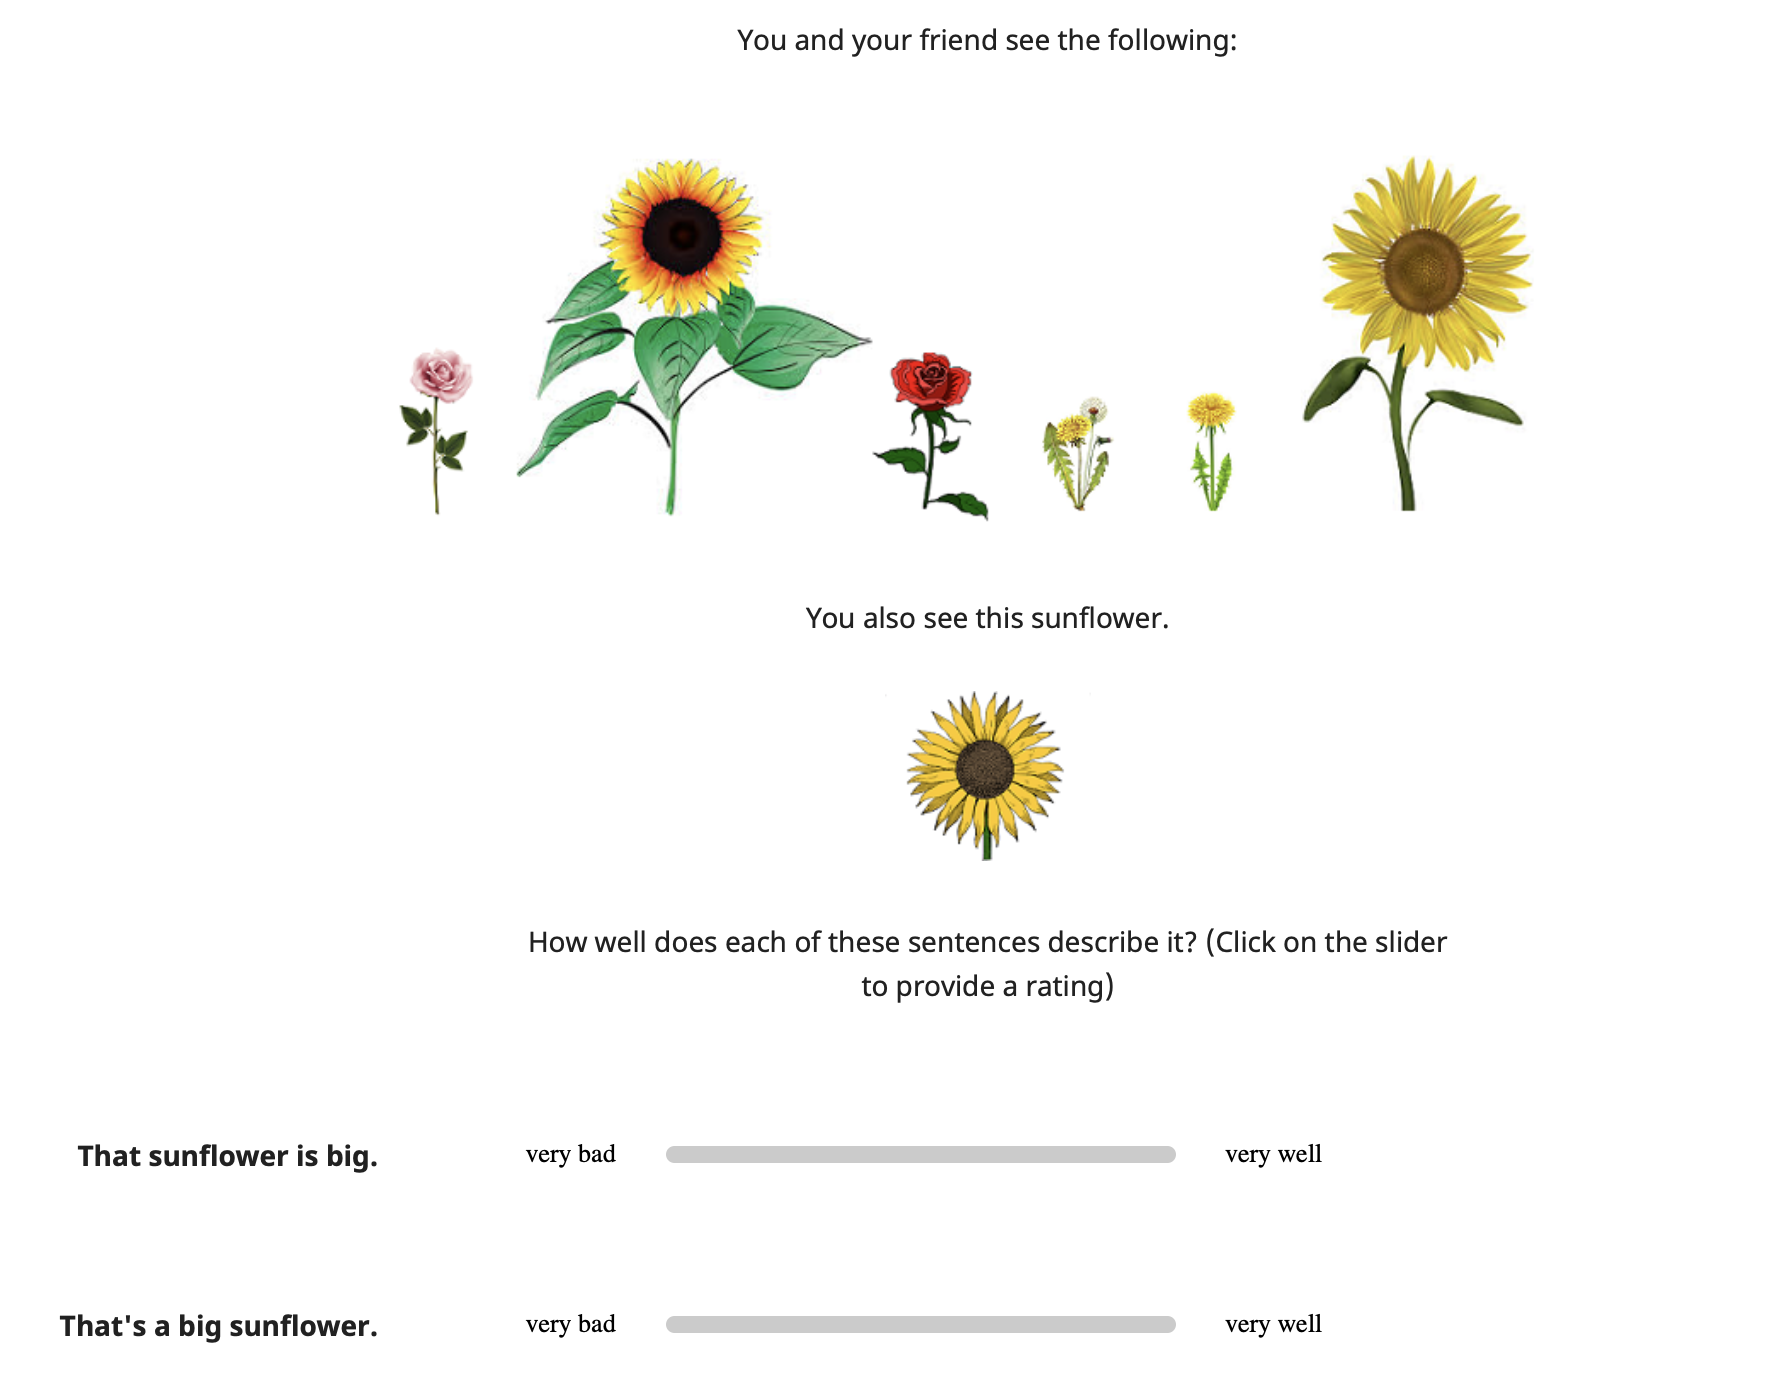
\includegraphics[width=0.7\linewidth]{main_rating_subN_big.png}
	\end{center}
	\caption{Example view of a sentence rating main trial: The critical noun is a subordinate target label of a large-subordinate category, appearing in the subject or predicate of the sentence.}
	\label{rating-main}
\end{figure*}
Then, participants completed six main trials (Fig.~\ref{rating-main}). Participants read “You and your friend see the following:” above a basic-level context picture (e.g., a group of flowers). In all experiments, the basic-level context pictures consisted of six members of the same basic-level category as the referent of the trial, including two other members of the same subordinate category as the referent, and four other objects. The six members consisted of two members of a large-subordinate, a medium-sized subordinate, and a small-subordinate category within the basic-level category each (e.g., the flower-context consisted of two subflowers, two roses and two dandelions; s. Fig.~\ref{rating-main}). The context was used to set the overall reference comparison class for the targets. It also set the visual reference frame.
Below, they read the sentence “You also see this SUB\_N”, where SUB\_N was the subordinate label of the target referent, which appeared depicted below, such that participants knew the subordinate category of the referent. The pictures depicted referents a little smaller than members of the same subordinate category in the context, such that the felicitous comparison class was pushed towards the basic-level category of the target.
Below, the question about the critical sentences appeared: “How well does each of the sentences describe it? (Click on the slider to provide a rating)”. Then, the two critical sentences appeared left of the sliders one below the other. The sliders ranged from “very bad” to “very well”. On every trial, in one of the sentences the noun appeared in the subject (e.g. “That N is \{big/small\}”), in the other in predicate position (“That’s a \{big/small\} N”). The order in which these syntactic conditions appeared was randomized between-subjects. 
On half of the trials, the noun was the basic-level target label (e.g., dog); on the other half it was the subordinate target label (e.g., Great Danes), balanced within-subjects. 
Participants saw each of the six possible contexts once, and for each context, one of the two possible targets (large-subordinate vs. small-subordinate category representative) was sampled, balanced within-participants (Table \ref{tab:stimuli}). 

The reference-predication trade-off hypothesis predicts that the effect of syntax on the rating will be more pronounced for sentences containing a subordinate noun than for sentences constaining a basic-level noun because a subordinate noun in predicate position would communicate an infelicitous comparison class for a normal-sized referent, while a basic-level predicate would be felicitous. That is, sentences with a basic-level noun in the predicate position are expected to receive a higher rating than sentences with a subordinate noun in the predicate, but a smaller difference in the ratings is expected for sentences with a noun in the subject position because either noun type can be felicitously used to pick out the referent. Given the specification of the statistical model (see Section~\ref{rating-results-section}), this prediction would be evidenced by a a negative credible estimate of the noun $\times$ syntax interaction.   

\subsection{Participants}
\rlgetvariable{myvars-rating.csv}{nSubj} participants were recruited and \rlgetvariable{myvars-rating.csv}{nExcludedTotal} were excluded for indicating a native language other than English, failing the practice trials or providing the same responses on every trial (see Appendix \ref{appendix}). The experiment took about 5 minutes and participants were compensated \$0.80. If partial data was missing from a participant, available data was used for analyses. 
\subsection{Results}
\label{rating-results-section}
For all reported experiments, maximal random effects structure licensed by the design was used \parencite{barr2013}. All statistical analyses were performed using the language R, in particular using the package \texttt{brms} for computing Bayesian regression models \parencite{Rteam2013, burkner2017advanced}.

A Bayesian linear mixed-effects regression model was fit for this experiment, predicting the sentence rating from the syntactic condition of the sentence (subject~vs.~predicate N), the noun type (basic-level~vs.~subordinate target label), their interaction and by-participant and by-target random intercepts and random effects of syntax, noun type and their interaction. \footnote{Model in \texttt{brm}-style syntax: \texttt{rating $\sim$ syntax * NP + (1 + syntax*NP | subject) + (1 + syntax*NP | target)}} 
Both predictors were sum-coded, coding both the subject-noun and the basic-level noun as 1 and the other levels as -1, respectively. Default priors were used.
An exploratory model including a main effect of syntactic condition order was also fit, revealing no effect of syntactic condition order, so the data was collapsed across the two conditions for further analyses. 

\begin{figure*}[t]
	\begin{center}
		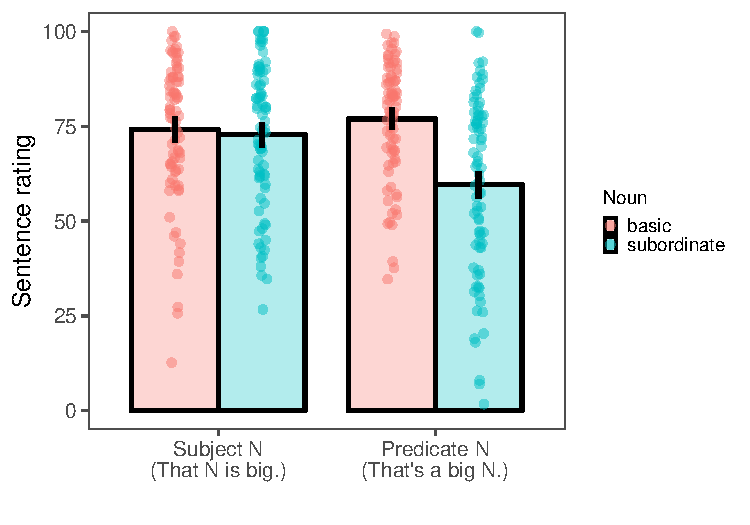
\includegraphics[width=0.7\linewidth]{expt-syntax-rating-prereg-bars-revised.pdf}
	\end{center}
 	\vspace{-0.3cm}
	\caption{Experiment 1 results: Mean ratings for how well sentences which differed in the syntactic position of the noun (x-axis)  and the noun-label (color) described a typically-sized referent (e.g., a Great Dane) in basic-level context.  Points represent participant means within condition. Error-bars denote bootstrapped 95\% confidence intervals (bootstrapping independent of random-effects structure).}
	\label{rating-results}
\end{figure*}
Consistent with predictions, participants substantially dispreferred sentences with a subordinate noun in the predicate compared to the subordinate position, but no effect of syntax was found for the basic-level nouns, as indicated by the syntax $\times$ noun-type interaction ($\beta = \rlgetnum{expt1_brm.csv}{Rowname}{syntax:NP}{Estimate}{2}  [\rlgetnum{expt1_brm.csv}{Rowname}{syntax:NP}{l.95..CI}{2}, \rlgetnum{expt1_brm.csv}{Rowname}{syntax:NP}{u.95..CI}{2}]$) (Fig. \ref{rating-results}).\footnote{All results report the mean and 95-\% Bayesian credible interval} 
Additionally, an overall preference for basic-level nouns ($\beta = \rlgetnum{expt1_brm.csv}{Rowname}{NP}{Estimate}{2} [\rlgetnum{expt1_brm.csv}{Rowname}{NP}{l.95..CI}{2},\rlgetnum{expt1_brm.csv}{Rowname}{NP}{u.95..CI}{2}] $) and the subject-noun syntactic structure ($\beta = \rlgetnum{expt1_brm.csv}{Rowname}{syntax}{Estimate}{2} [\rlgetnum{expt1_brm.csv}{Rowname}{syntax}{l.95..CI}{2}, \rlgetnum{expt1_brm.csv}{Rowname}{syntax}{u.95..CI}{2}] $) was found. Furthermore, a relatively high by-target variance revealed that some items received overall lower ratings, possibly due to differing namability or typicality of the items (by-target intercept: $\beta = \rlgetnum{expt1_random_brm.csv}{Rowname}{sd(Intercept)}{item.Estimate}{2} [\rlgetnum{expt1_random_brm.csv}{Rowname}{sd(Intercept)}{item.l.95..CI}{2}, \rlgetnum{expt1_random_brm.csv}{Rowname}{sd(Intercept)}{item.u.95..CI}{2}]$). A relatively high by-participant variation indicated differences in overall rating preferences (by-subject intercept: $\beta = \rlgetnum{expt1_random_brm.csv}{Rowname}{sd(Intercept)}{submission_id.Estimate}{2} [\rlgetnum{expt1_random_brm.csv}{Rowname}{sd(Intercept)}{submission_id.l.95..CI}{2}, \rlgetnum{expt1_random_brm.csv}{Rowname}{sd(Intercept)}{submission_id.u.95..CI}{2}]$).
Finally, an exploratory analysis including a target size predictor (small-subordinate vs. large-subordinate category) did not reveal any size-effects on the rating. 

To sum up, the sentence rating experiment showed that participants are sensitive to the position and the type of the noun, dispreferring sentences where a noun that provided an infelicitous comparison appeared predicatively.  

\section{Experiment 2: Noun Production Experiment}    

%classification of responses
%results: main, by-participant / by-item, by-size  

The goal of the noun production experiment was to investigate whether participants produce nouns of different categories in a free-production setting, given different syntactic frames.  The noun slot of the critical sentences in the main trials appeared either in the subject position (e.g., in “That \_ is \{big/small\}“) or in the predicate position (e.g., in “That’s a \{big/small\} \_”), manipulated between-subjects. 

\begin{figure*}[t]
	\begin{center}
		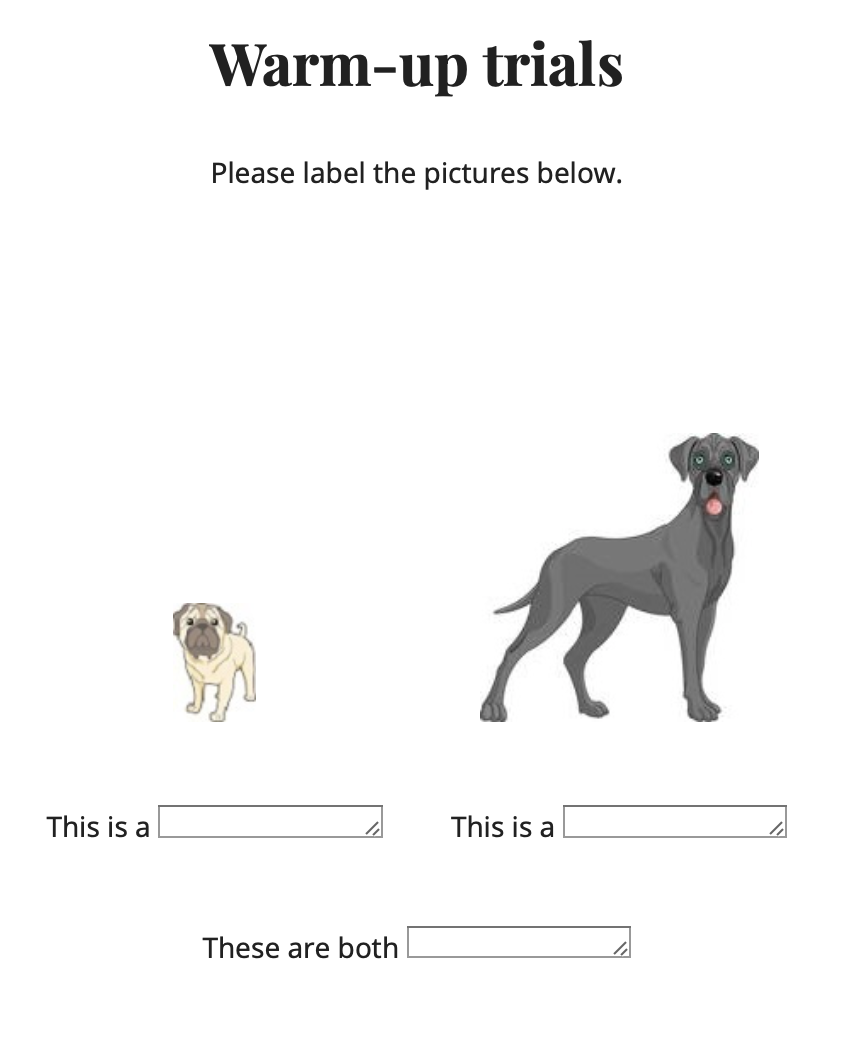
\includegraphics[width=0.5\linewidth]{warmup_dogs.png}
	\end{center}
	\caption{Example view of the noun production warm-up trial: Participants have to label a large-subordinate (Great Dane, right) and a small-subordinate target (pug, left) for the dogs-category.}
	\label{warmup-production}
\end{figure*}
Participants completed two experimental blocks, each consisting of three warm-up trials and three main trials. In the warm-up trials participants familiarized themselves with the subordinate categories used in the main trials. They saw pictures of a member from a large-subordinate and a small-subordinate category within one of the basic-level categories used in the main trials within the same block (e.g., a Great Dane and a pug) (Fig. \ref{warmup-production}). Participants were prompted to provide labels for these pictures. Below they were prompted to provide a common label for both pictures (i.e., dogs), so that they were 'warmed-up' to provide lables of different categories. They were provided feedback for the labels and could proceed upon adjusting their labels to correct responses. The number of attempts participants needed until they filled-in the correct labels was recorded. In this experiment, four additional subordinate categories were used, which can be found in Table \ref{tab:stimuli} marked with *. For each participant, six out of ten possible contexts were sampled. Three of these contexts and their corresponding targets appeared in the first experimental block, and the other three in the second. The trial order within the warm-up block and the main block was randomized. 

\begin{figure*}[t]
	\begin{center}
		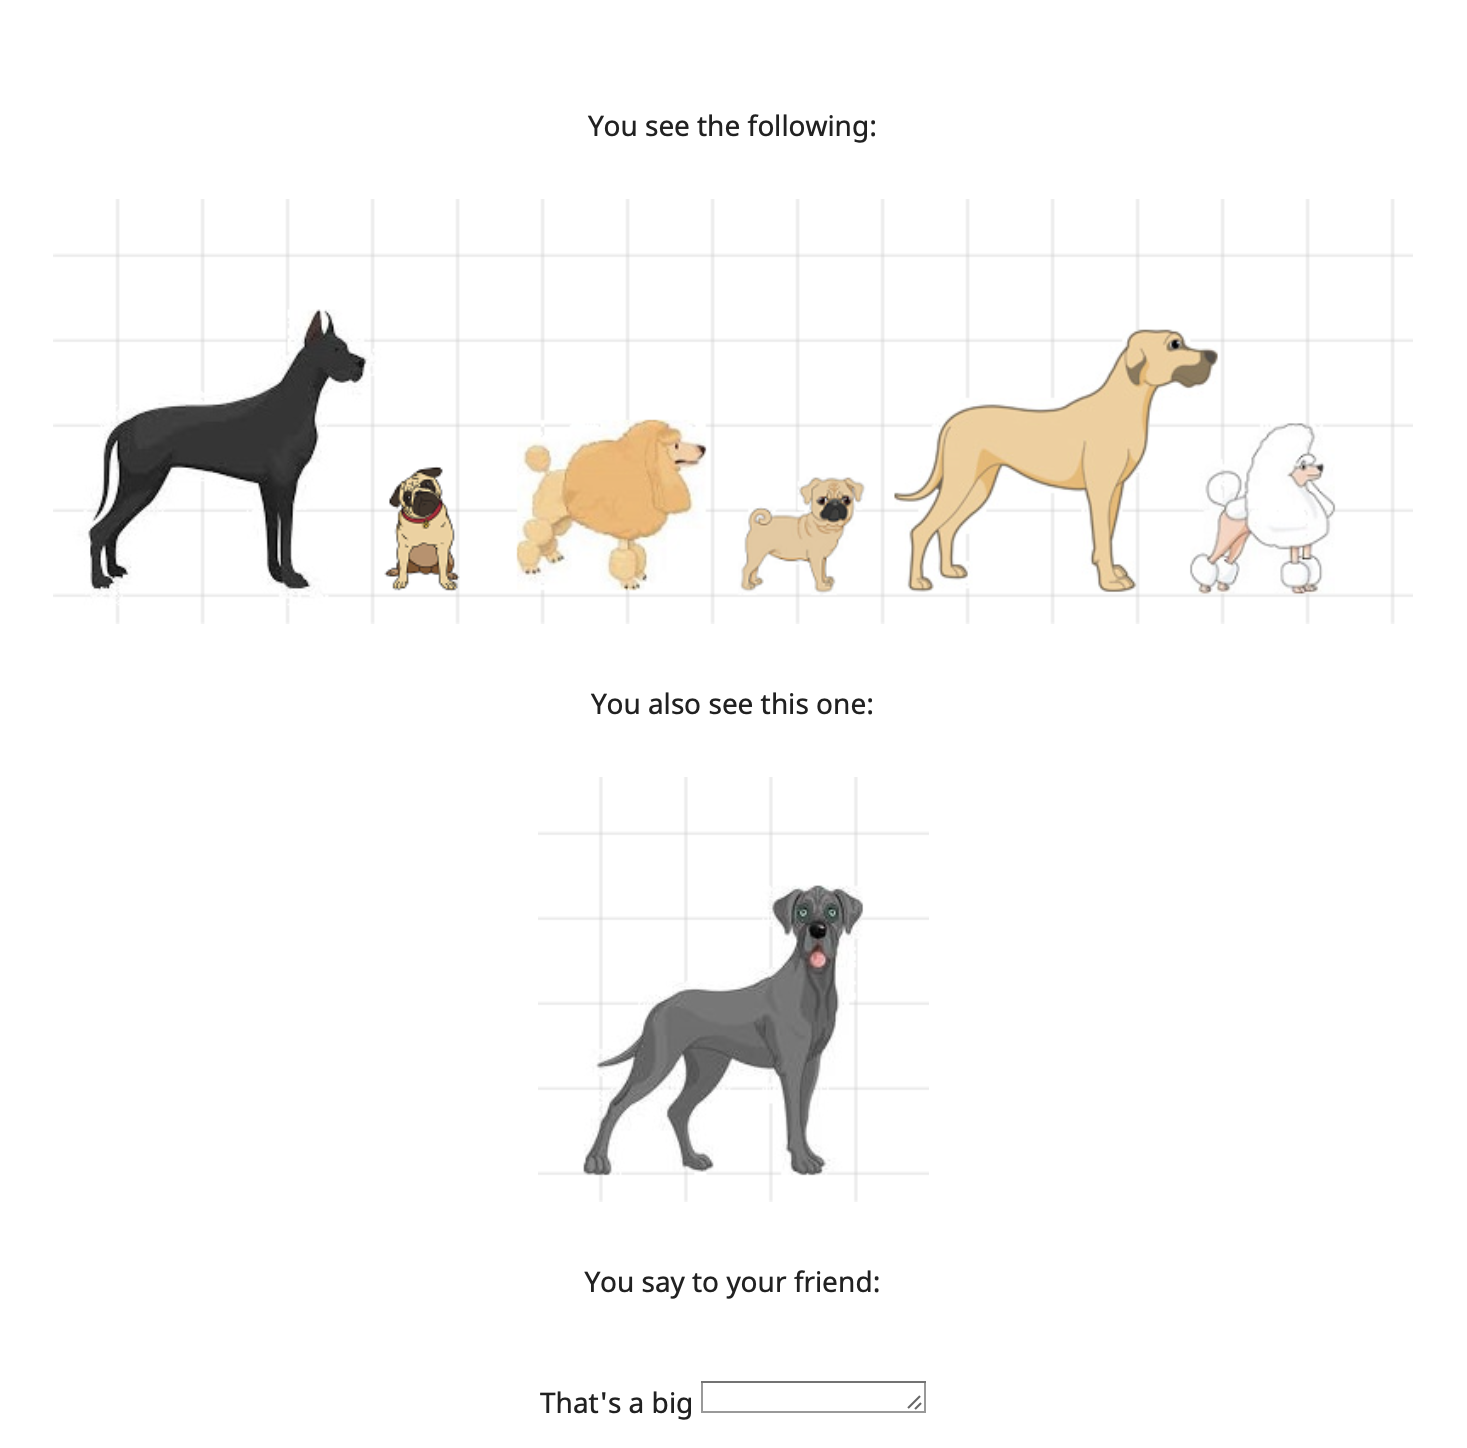
\includegraphics[width=0.7\linewidth]{main_prod_predN_big.png}
	\end{center}
	\caption{Example view of the noun production main trial: Participants fill-in the noun in the predicate position of a sentence describing a large-subordinate target.}
	\label{main-production}
\end{figure*}
On the main trials, participants read: “You see the following:” above a basic-level context picture, akin to the contexts used in Experiment 1. Below, they read “You also see this one:” and saw a picture of the target referent. Then they read: “You say to your friend:”, prompting them to fill-in the missing noun in the sentence: for the subject-noun condition, the template was “That\_\_ is \{big/small\}”, for the predicate-noun condition, the template to be completed was “That’s a \{big/small\} \_\_ “ (Fig. \ref{main-production}).  
The size of the target referent was balanced within-participants: on three trials, participants saw referents from a small-subordinate category, and on three, they saw referents from a large-subordinate category. For each context, participants saw only one of the possible targets (e.g., the large or the small subordinate target).

The reference-predication hypothesis predicts that speakers sensitive to listeners' expectations about acomplishment of communicative goals should be more likely to produce basic-level target labels than subordinate target labels in the predicate compared to the subject position. A positive credible regression coefficient for the effect of syntax would confirm this prediction, indicating a hisher proportion of basic-level responses in the predicate compared to the subject position. 

\subsection{Participants}
\rlgetvariable{myvars-np.csv}{nSubj}  participants were recruited, and \rlgetvariable{myvars-np.csv}{nExcludedTotal}  were excluded for indicating a native language other than English or for failing the warm-up trials. The exclusion criterion was taking more than four attempts on any warm-up trial to provide the expected answer upon correction. The experiment took about 7 minutes and participants were compensated \$1.00. 
 
\subsection{Results}
\begin{figure*}[t]
	\begin{center}
		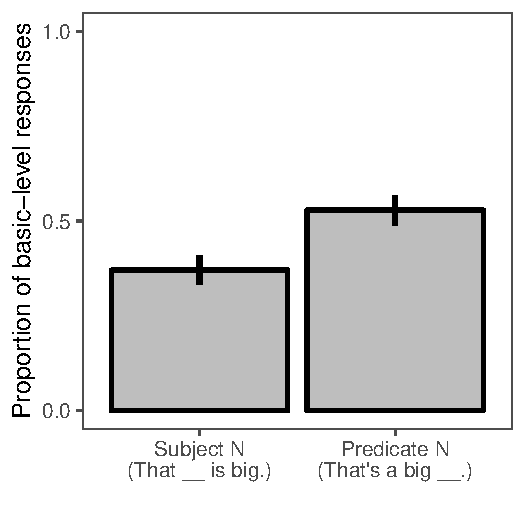
\includegraphics[width=0.5\linewidth]{expt-np-prod-prereg-bars-revised.pdf}
	\end{center}
	\vspace{-0.3cm}
	\caption{Experiment 2 results: Proportions of freely-produced basic-level labels (e.g., \emph{dog}) in different syntactic frames (x-axis) when the referent was a typically-sized member of a subordinate category (e.g., a normal-sized Great Dane). Error-bars denote 95\% bootstrapped confidence intervals.}
	\label{production-results}
\end{figure*}
The responses provided by participants were categorized manually into basic-level or subordinate-level labels of the targets, disregarding the noun number and spelling mistakes. 5 responses were superordinate referent labels (i.e., more general labels like 'animals') and were collapsed with basic-level labels. 16 (1.4\%) uncategorizable responses were excluded from analysis (see Appendix \ref{appendix} for all responses). 
A logistic generalized mixed-effects Bayesian regression model was fit, regressing the response category (basic-level~vs.~subordinate target label) against the syntax of the sentence (subject-N~vs.~predicate-N), random by-participant and by-referent intercepts and random by-referent slope effects of syntax.\footnote{In brm-style syntax: \texttt{response\_category $\sim$ syntax + (1 | subject) + (1 + syntax | target)}}
Default priors were used. The predictor was deviation-coded, coding predicate-N syntax as 0.5 and subject-N syntax as -0.5.

Consistent with predictions, a strong effect of syntactic position of the noun was found, indicating that participants were more likely to use basic-level labels in the predicative position ($\beta = \rlgetnum{expt2_brm.csv}{Rowname}{syntax_contr}{Estimate}{2} [\rlgetnum{expt2_brm.csv}{Rowname}{syntax_contr}{l.95..CI}{2}, \rlgetnum{expt2_brm.csv}{Rowname}{syntax_contr}{u.95..CI}{2}]$) (Fig. \ref{production-results}). That is, participants were more likely to provide the noun matching the felicitous comparison class in the predicate position, but more likely to use the noun with higher referential utility in the subject.    
As expected, an exploratory model including a main effect of referent size (large-subordinate vs. small-subordinate category) did not reveal any differences between target types. By-target random effects revealed that participants were generally more likely to produce subordinate labels for some targets than for others (by-target intercept: $\beta = \rlgetnum{expt2_random_brm2.csv}{Rowname}{Intercept}{target.Estimate}{2} [\rlgetnum{expt2_random_brm2.csv}{Rowname}{Intercept}{target.l.95..CI}{2}, \rlgetnum{expt2_random_brm2.csv}{Rowname}{Intercept}{target.u.95..CI}{2}]$). For example, participants were very likely to produce the subordinate label for the swan-item, possibly due to namability effects.

The noun production experiment showed that speakers are sensitive to the syntactic structure of the sentence and flexibly adjust their noun choices in order to communicate a felicitous comparison class, when presented with a free-production task.  
 
 
\section{Experiment 3: Comparison Class Inference Experiment}
The two previous experiments support the reference-predication trade-off view, by showing that participants disprefer sentences like “That’s a big Great Dane” in order to describe a normal-sized Great Dane, but accept either target label in the sentence subject. The goal of this comparison class inference experiment was to measure comparison class inferences more directly, presenting participants with sentences they had to paraphrase. The types of inferred comparison classes were investigated, as influenced by the position of the critical noun in the sentence (subject.~vs.~ predicate), the type of noun (basic-level~vs.~subordinte~vs.~'one') and the visual context of the sentence (basic-level~vs.~subordinate context). All three factors were manipulated within-subjects.

In this experiment, participants first completed a comparison class paraphrase practice trial, akin to the paradigm employed in the main trials. Participants were told that on the main trials they will see a sentence containing a word that is relative, and their task will be to figure out what this word is relative to. They read an example task: “Speaker A: ‘The Empire State building is tall.’ What do you think speaker A meant?”. Below they saw a paraphrase template where they provided the inferred comparison class of the adjective \emph{tall}: “The Empire State building is tall relative to other\_\_” (blank to be completed with the inferred comparison class). Participants were provided feedback on their response and had to correct it to one of the possible options among \{buildings, skyscrapers, houses, constructions\}. 
Then, participants completed two blocks consisting of labeling warm-up trials and main paraphrase trials. Three of the six basic-level categories used in this experiment were sampled for the first block, with the respective subordinate category members appearing in the warm-up trials, the other three categories appeared in the second block (Table \ref{tab:stimuli}). These labeling warm-up trials are of the same kind as in Experiment 2 (Fig. \ref{warmup-production}). 

\begin{figure*}[t]
	\begin{center}
		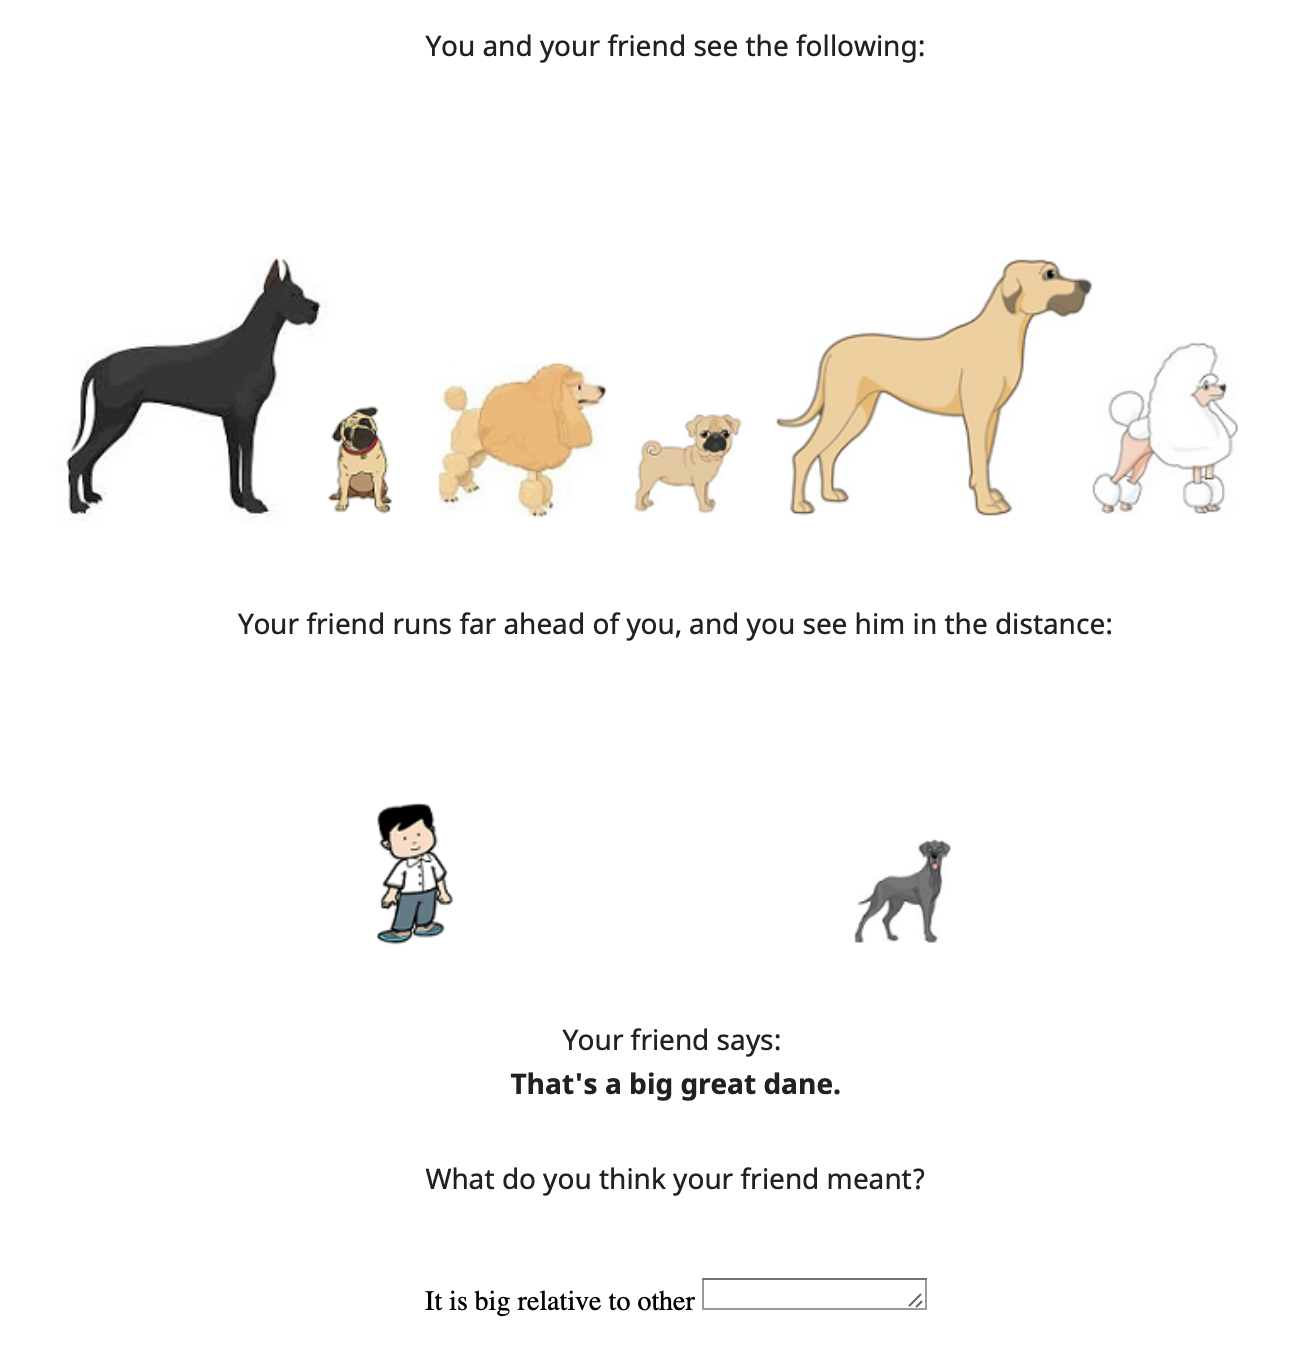
\includegraphics[width=0.7\linewidth]{main_cci_basicContext_predSubN_big.png}
	\end{center}
	\caption{Example view of a comparison class inference main trial: Participants paraphrased the critical utterance with a subordinate noun in predicate position, which appeared in basic-level context, describing a large-subordinate target.}
	\label{main-cci}
\end{figure*}
For the main trials there were basic-level and subordinate-level contexts for each possible referent. Basic-level contexts were identical to the contexts of respective categories in Experiment 1 and Experiment 2 (Figs.~\ref{main-production}, \ref{rating-main}); the subordinate contexts consisted of six other representatives of the same subordinate category as the target referent. For example, the subordinate context for a Great Dane consisted of a picture of a group of six other Great Danes. \pt{add example picture} Within each main trial block, there were six trials, wherein for each of the three sampled categories, one possible referent appeared in the corresponding basic-level context (e.g., for the category flowers, the sunflower appeared in basic-level flower context), and the other possible referent appeared in the corresponding subordinate context (i.e., then the daisy appeared in subordinate daisies-context). 
The referent was described by a critical sentence in which the noun could appear in the subject or in the predicate of the sentence. The noun could be either the basic-level (e.g., dog) or the subordinate label of the referent (e.g., Great Dane). Furthermore, a baseline condition with an anaphoric ‘one’ in the noun position was included, in order to measure the baseline influence of the visual context on comparison class inference: the anaphora is most likely to be resolved contextually, meaning "dog" in the basic-level context and "Great Dane" in subordinate context \parencite{goldberg2017one}. Crossing the visual context (basic vs. subordinate), the syntax (subject-N vs. predicate-N) and the possible nouns (basic vs. subordinate vs. ‘one’) results in a 2x2x3 design, yielding 12 unique conditions.\footnote{Due to my coding mistake, the conditions were balanced at the level of individual factors. That is, each participant saw six trials in basic-level and six trials in subordinate context, six trials in the subject and six in the predicate condition, as well as four trials in each noun-condition. However, participants potentially did not see all 12 possible combination of these factors.}
Each participant saw a total of 12 main trials.   

On main trials, participants read “You and your friend see the following:” above a context picture  (Fig. \ref{main-cci}). Below, they read: “Your friend runs far ahead of you, and you see him in the distance:”. The illusion of distance was created contextually in order to disguise the perceptual size of the target referent and push participants towards inferring the size of the referent from the sentence, rather than perceptually. This illusion was supported by the picture appearing below, wherein the small target referent was depicted next to a small person (as compared to the context, i.e., appearing in distance). Below, participants read: “Your friend says:”, followed by the critical sentence. Participants were asked “What do you think your friend meant?”, followed by the paraphrase template “It is \{big/small\} relative to other \_\_”, blank to be completed with the inferred comparison class. The order of context, noun and syntax conditions was randomized for each participant.

When participants don’t have access to visually assessing the size of a referent and need to infer the comparison class from the sentence, they might be more sensitive to linguistic cues like the sentence structure. According to the reference-predication hypothesis, they would be more likely to take the noun as a cue to the comparison class when the noun appears in the predicate of that sentence, than when it appears in the subject. 
When the noun appears in the subject, comparison class inference can be driven by other pragmatic inferences, e.g., by world knowledge and visual context. If this is true, more basic-level comparison classes should be inferred from sentences appearing in basic-level context, compared to subordinate context. A credible positive regression coefficient for the effect of context would support this prediction. Additionally, inferences drawn from the anaphoric 'one' which is the baseline condition for the effects of visual context are then expected to mirror this difference, such that more basic-level comparison class should be inferred in the basic-level context than in the subordinate context, evidenced by a credible positive estimate for the respective contrast (cf. Section~\ref{cci-results-text}; \textcite[cf.][]{goldberg2017one}).
 
In particular, nouns with a high referential utility (e.g., subordinate target labels given a basic-level set of distractors, \textcite[cf.][]{graf2016animal}) should highlight the main reference-predication prediction, by providing strong referential cues in the subject, but potentially signalling a comparison class different from prior world knowledge and perceptual context in the predicate. That is, participants are expected to infer more subordinate comparison classes (i.e., less basic-level ones) from predicate subordinate nouns than from subject subordinate nouns. In contrast, a smaller difference in comparison classes inferred from basic-level nouns in different positions is expected, since this noun in the predicate would signal the basic-level comparison class, and pragmatic inferences driving comparison class inference when this noun appers in the subject would also suggest the basic-level comparison class (e.g., given world knowledge and especially the basic-level context). 
For this prediction to be supported statistically, a credible positive syntax $\times$ noun interaction regression estimate is expected.
 
On the contrary, if comparison class inference was completely driven by the noun of the sentence or other purely syntactic or semantic properties discussed in Chapter \ref{chapter02}, no interpretative differences should be observed when the same sentences occur in different perceptual contexts. In this case, no credible effect of context will be observed. Taking an opposite point of view, another conceivable mechanism for gradable adjective interpretation wherein the perceptual context only supplies the comparison class would predict identical inferences drawn from sentences involving different nouns or different syntactic structure. In this case, no credible effects of noun type or syntax should be observed. 

\subsection{Participants}
\rlgetvariable{myvars-infer.csv}{nSubj} participants were recruited and \rlgetvariable{myvars-infer.csv}{nExcludedTotal} were excluded for indicating a native language other than English, or failing either the comparison class inference practice trial or the labeling warm-up trials more than four times upon correction. The experiment took about 9 minutes and participants were compensated \$1.20. 
\subsection{Results}
\label{cci-results-text}
%by-target / by-participant variation
%by-size?
\begin{figure*}[t]
	\begin{center}
		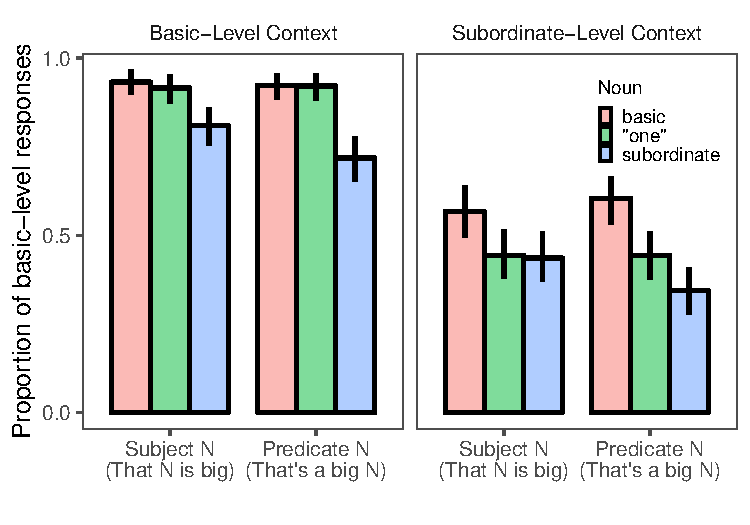
\includegraphics[width=0.7\linewidth]{expt3-cc-inference-revised.pdf}
	\end{center}
	\vspace{-0.3cm}
	\caption{Experiment 3 results: Proportions of inferred comparison classes in terms of basic-level responses (e.g.,~“...big relative to other dogs”), depending on syntactic position of the noun (x-axis), noun-label (color), and context (facets).
		Context strongly modulated the comparison class (left~vs.~right panel). 
		The noun additionally provided a cue to the comparison class (red~vs.~blue) bars, regardless of syntactic position. 
		The effect of noun (red~vs.~blue) is modulated by syntax. 
		Error-bars denote bootstrapped 95\% confidence intervals.}
	\label{cci-results}
\end{figure*}
Participants’ responses were manually classified into basic-level and subordinate comparison classes. 4 superordinate comparison classes were collapsed with the basic-level responses. 39 (1.6\%) uncategorizable responses were excluded from the analysis (s. Appendix \ref{appendix}). 
A Bayesian logistic mixed-effects regression model was used, regressing the response category against the syntactic condition (subject-N vs. predicate-N), the noun category (basic vs. subordinate vs. ‘one’), the context (basic vs. subordinate), their two-way and three-way interactions and maximal random effect structure appropriate for this experimental design.\footnote{In brm-style syntax: \texttt{response\_category $\sim$ syntax*NP*context + (1 + syntax + NP + context || subject) + (1 + syntax*NP*context || target)}. Correlations of random effects were set to 0 for computational tractability.} Default priors were used.
The predictors were sum-coded: predicate-N and basic-level context were coded as 1, subject-N and subordinate context as -1; the basic-level and the subordinate noun-levels were coded against the baseline anaphoric 'one'. 

The results indicate that participants flexibly adjust the inferred comparison class according to many factors. First and foremost, a large effect of visual context going above and beyond other factors was found ($\beta = \rlgetnum{expt3_full_brm_revised2.csv}{Rowname}{context_sum}{Estimate}{2} [\rlgetnum{expt3_full_brm_revised2.csv}{Rowname}{context_sum}{l.95..CI}{2},  \rlgetnum{expt3_full_brm_revised2.csv}{Rowname}{context_sum}{u.95..CI}{2}]$; Fig.~\ref{cci-results}, left~vs.~right facets), supported by the inferences drawn from the baseline condition anaphoric ‘one’ ($\beta = \rlgetnum{expt3_3way_full_contrasts_wProbs.csv}{Rowname}{context_one_v_mean}{mean}{2} [\rlgetnum{expt3_3way_full_contrasts_wProbs.csv}{Rowname}{context_one_v_mean}{X.95.}{2}, \rlgetnum{expt3_3way_full_contrasts_wProbs.csv}{Rowname}{context_one_v_mean}{u95.}{2}]$; Fig. \ref{cci-results}, green bars in the left~vs.~right facet): participants were appreciably more likely to infer basic-level comaprison classes given a basic-level context, compared to a subordinate context. Furthermore, an effect of the noun on inferred comparison classes regardless of its position in the sentence was found: participants were more likely to infer basic-level comparison classes from basic-level nouns than from subordinate nouns ($\beta = \rlgetnum{expt3_3way_full_contrasts_wProbs.csv}{Rowname}{basic_v_sub}{mean}{2} [\rlgetnum{expt3_3way_full_contrasts_wProbs.csv}{Rowname}{basic_v_sub}{X.95.}{2}, \rlgetnum{expt3_3way_full_contrasts_wProbs.csv}{Rowname}{basic_v_sub}{u95.}{2}$]). The noun-effects can be observed on top of effects of the visual context indicated by the baseline condition 'one': participants inferred more basic-level comparison classes from basic-level nouns that from 'one', and less from subordinate nouns that from 'one' (basic-level~vs.~'one': $\beta = \rlgetnum{expt3_3way_full_contrasts_wProbs.csv}{Rowname}{basic_v_one}{mean}{2} [\rlgetnum{expt3_3way_full_contrasts_wProbs.csv}{Rowname}{basic_v_one}{X.95.}{2}, \rlgetnum{expt3_3way_full_contrasts_wProbs.csv}{Rowname}{basic_v_one}{u95.}{2}]$; and subordinate~vs.~'one': $\beta = \rlgetnum{expt3_3way_full_contrasts_wProbs.csv}{Rowname}{sub_v_one}{mean}{2} [\rlgetnum{expt3_3way_full_contrasts_wProbs.csv}{Rowname}{sub_v_one}{X.95.}{2}, \rlgetnum{expt3_3way_full_contrasts_wProbs.csv}{Rowname}{sub_v_one}{u95.}{2}]$). 
Notably, the subordinate comparison class was the minority response even given a subordinate noun in the basic-level context, speaking against a compositional view of adjective comparison classes, wherein the noun would always set the comaprison class (Fig. \ref{cci-results}; blue bars, left facet). Even in the subordinate context inferences drawn from the subordinate noun were not exclusively subordinate comparison classes, indicating a basic-level bias \parencite[Fig.~\ref{cci-results}; blue bars, right facet; cf.][]{rosch1976, graf2016animal}. 

Crucially, a credible syntax-by-noun interaction was found, supporting predictions provided by the reference-predication trade-off hypothesis: more subordinate comparison classes were inferred from subordinate nouns appearing in predicate position than in the subject position, compared to basic-level nouns (red~vs.~blue bars $\times$ x-axis; $\beta = \rlgetnum{expt3_3way_full_contrasts_wProbs.csv}{Rowname}{syntax_basic_v_sub}{mean}{2} [\rlgetnum{expt3_3way_full_contrasts_wProbs.csv}{Rowname}{syntax_basic_v_sub}{X.95.}{2}, \rlgetnum{expt3_3way_full_contrasts_wProbs.csv}{Rowname}{syntax_basic_v_sub}{u95.}{2}]$). Examining the interaction by-noun, preliminary evidence was found that the interaction is primarily driven by the subordinate noun: a $\rlgetnum{expt3_3way_full_contrasts_wProbs.csv}{Rowname}{syntax_sub_v_one}{prob_lt_0}{1}$\% probability was found that the subordinate-N~vs.~'one' $\times$ Syntax interaction term was less than 0 (i.e., more subordinate comparison classes were inferred when the noun was in the predicate; $\beta = \rlgetnum{expt3_3way_full_contrasts_wProbs.csv}{Rowname}{syntax_sub_v_one}{mean}{2} [\rlgetnum{expt3_3way_full_contrasts_wProbs.csv}{Rowname}{syntax_sub_v_one}{X.95.}{2}, \rlgetnum{expt3_3way_full_contrasts_wProbs.csv}{Rowname}{syntax_sub_v_one}{u95.}{2}]$), in contrast to only a $\rlgetnum{expt3_3way_full_contrasts_wProbs.csv}{Rowname}{syntax_basic_v_one}{prob_gt_0}{1}$\% probability of the basic-N~vs.~'one' $\times$ Syntax interaction being greater than 0 (i.e., more basic-level comparison classes inferred when the noun was in the predicate; $\beta = \rlgetnum{expt3_3way_full_contrasts_wProbs.csv}{Rowname}{syntax_basic_v_one}{mean}{2} [\rlgetnum{expt3_3way_full_contrasts_wProbs.csv}{Rowname}{syntax_basic_v_one}{X.95.}{2}, \rlgetnum{expt3_3way_full_contrasts_wProbs.csv}{Rowname}{syntax_basic_v_one}{u95.}{2}]$). This is consistent with the reference-predication trade-off hypothesis, predicting that an effect of syntax is more pronounced for nouns with higher referential utility, which is generally the case for subordinate compared to basic-level nouns, especially in the basic-level context \parencite[cf.][]{graf2016animal}. This effect was even more pronounced under an exploratory model, assuming only a two-way syntax-by-noun interaction and a main effect of context: the probability was $\rlgetnum{expt3_2way_full_contrasts_wProbs.csv}{Rowname}{syntax_sub_v_one}{prob_lt_0}{1}$\% for the subordinate noun~vs.~'one' $\times$ Syntax estimate to be less than 0.\footnote{Exploratory model: \texttt{response\_category $\sim$ syntax*NP + context + (1 + syntax + NP + context || subject) + (1 + syntax*NP + context || target)}}

Taking the reference-predication trade-off hypothesis even further, another exploratory analysis suggested that participants might consider informational functions of the noun irrespective of the syntactic position. For instance, when a noun in the subject is referentially uninformative they might reason that this noun too is intended for predication. In particular, the subordinate context yields the basic-level target label referentially uninformative (all members of context can be described by the basic-level noun), such that listeners might reason about the presence of the noun as intended to convey the comparison class when it appears in both subject or predicate position. In line with this idea, in the subordinate context condition a higher rate of basic-level comparison classes was inferred from the basic-level noun comapred to 'one' ($\rlgetnum{expt3_subContext.csv}{Rowname}{basic_v_one}{prob_gt_0}{1}$\% of the credible interval of the basic~vs.~'one' estimate was greater than 0: $\beta = \rlgetnum{expt3_subContext.csv}{Rowname}{basic_v_one}{mean}{2} [\rlgetnum{expt3_subContext.csv}{Rowname}{basic_v_one}{X.95.}{2}, \rlgetnum{expt3_subContext.csv}{Rowname}{basic_v_one}{u95.}{2}]$; Fig. \ref{cci-results}; red~vs.~green bars, right facet), indicating an effect of the basic-level noun going beyond contextual resolution of this referentially underspecified expression, as in case of 'one'.
%and more subordinate comparison classes were inferred from subordinate labels comapred to 'one' ($\rlgetnum{expt3_subContext.csv}{Rowname}{sub_v_one}{prob_lt_0}{1}$\% of the credible interval of the subordinate~vs.~'one' estimate was smaller than 0: $\beta = \rlgetnum{expt3_subContext.csv}{Rowname}{sub_v_one}{mean}{2} [\rlgetnum{expt3_subContext.csv}{Rowname}{sub_v_one}{X.95.}{2}, \rlgetnum{expt3_subContext.csv}{Rowname}{sub_v_one}{u95.}{2}]$;Fig. \ref{cci-results}; blue~vs.~green bars, right facet), across syntactic frames.
\footnote{These contrasts were computed on data subsetted by context}
The data observed in the basic-level context is also consistent with the hypothesis that the referentially uninformative noun in the subject signals the comparison class, but the referentially-uninformative basic-level label condition and the baseline 'one' are both subject to a ceiling effect and hence leave no room for any effects beyond baseline.  

These empirical results provide a comprehensive picture of syntactic and pragmatic effects contributing to comparison class inference. In particular, this experiment shows that the same utterances are interpreted differently in distinct contexts, as evidenced by the large effect of context. This speaks against purely syntactic or semantic views arguing that meaning of utterances is fully specified by their words (as discussed in Section \ref{2.3.}). Furthermore, the influence of the noun in the utterance independent of context and syntactic position confirms that the noun is a salient cue to the comparison class, yet insufficient on its own to account for interpretative differences observed. Finally, evidence consistent with the reference-predication hypothesis is found, suggesting that humans integrate the referential utility with contextual cues when reasoning about the contribution of the noun to the comaprison class (as shown by the noun $\times$ syntax interaction). The data suggests that one-dimensional theories of gradable adjective interpretation do not account for flexible comparison class inference; humans integrate both pragmatic and syntactic information to felicitously use gradable adjectives across different contexts. 

\section{Experiment 4: Direct Modification Experiment} 
However, in order to keep a simple operationalization of the reference-predication distinction, a potential confound was introduced in experiments 1-3. The position of the noun was perfectly confounded with whether the noun was directly syntactically modified by the adjective (predicate-N condition) or not (subject-N condition). Therefore, experiments 1-3 did not allow to rule out that the observed interpretative differences were not due to the differing modification, as discussed in Section \ref{2.3.}.  Yet the reference-predication trade-off view predicts that referential pressure takes off predicational weight from the noun used for reference and therefore decreases its strength in constraining the comparison class, independent of the syntactic modification because informational goals are suggested to be the primary driving force above syntactic phenomena. This prediction was investigated in this direct-modification experiment.

That is, the main idea of this study was to manipulate the position of the noun while the modification was constant across the positions. Therefore, in critical trials the position of the critical noun in the sentence was varied and the noun was always directly modified by the adjective \textit{big} or \textit{small} (i.e., 'big Great Dane', 'small pug'). The critical nouns were always subordinate referent labels. In order to create maximally symmetric syntactic manipulations of the critical sentences, a second noun was used which described a visually salient feature of the referent. For example, the referents for one of the dog contexts were prize-winners, as indicated by prize-bows depicted on the referents (Table~\ref{stims:e4})). So the critical sentence was either “That prize-winner is a big Great Dane” (predicate-N) or “That big Great Dane is a prize-winner” (subject-N). For the same reason nouns were chosen to describe this feature as opposed to e.g.~adjectives ("That big Great Dane is polka-dotted"~vs.~??"That polka-dotted is a big Great Dane"). The features were chosen such that they were visually accessible, describable by a noun and would be part of the referent.   
The referents appeared in a basic-level context, which included two other members of the same subordinate category as the referent, and two other individuals with the feature described by the second noun of the sentence: e.g., in the dog-context there were two other prize-winners (Fig.~\ref{double-mod-main}). Because the reference-predication trade-off is based on explaining away a noun via its potential referential use, through this contextual manipulation the referential utilities of the two nouns of the sentence were equal, such that only the noun’s syntactic position and combination with the deictic ‘that’ could provide a cue towards referential intention. Therefore, the critical subordinate noun is expected to constrain the inferred comparison class more strongly when it appears in the predicate of the sentence rather than in the subject. 

\begin{table}[t]
	\small{
		\begin{center}
			\caption{E4 experimental items: each basic-level context had two potential targets from an either saliently small or saliently big subordinate category within the basic-level class. Each category had a corresponding context cover story which was comleted by "...and you see the following:". The referents had an additional visually salient feature, described by the second noun in critical sentences (N2).}
			\label{stims:e4}
			\vskip 0.12in
			\fontsize{10}{11}\selectfont
			\setlength{\extrarowheight}{.5em}
			\begin{tabularx}{\textwidth}{>{\hsize=.6\hsize}X>{\hsize=.8\hsize}X>{\hsize=.8\hsize}X>{\hsize=2\hsize}X>{\hsize=.8\hsize}X}
				\hline
				Basic-level \newline category & Smaller \newline referent & Bigger \newline referent & Context & Visual \newline feature / N2\\
				\hline
				Dogs & Pug & Great Dane & You and your friend are at a pet show. & prize-winner \\
				Dogs & Chihuahua & Doberman & You and your friend are at an animal training ground. & service-animal\\
				Birds & Hummingbird & Eagle & You visit your friend who works at an animal shelter. & rescue  \\
				Flowers & Dandelion & Sunflower & You and your friend are at their garden. & gift\\
				Trees & Bonsai & Redwood & You and your friend walk to their cabin in a park for the first time. You want to memorize the path. & landmark\\
				\hline     
			\end{tabularx}
		\end{center}
	}
\end{table}

\begin{figure*}[t]
	\begin{center}
		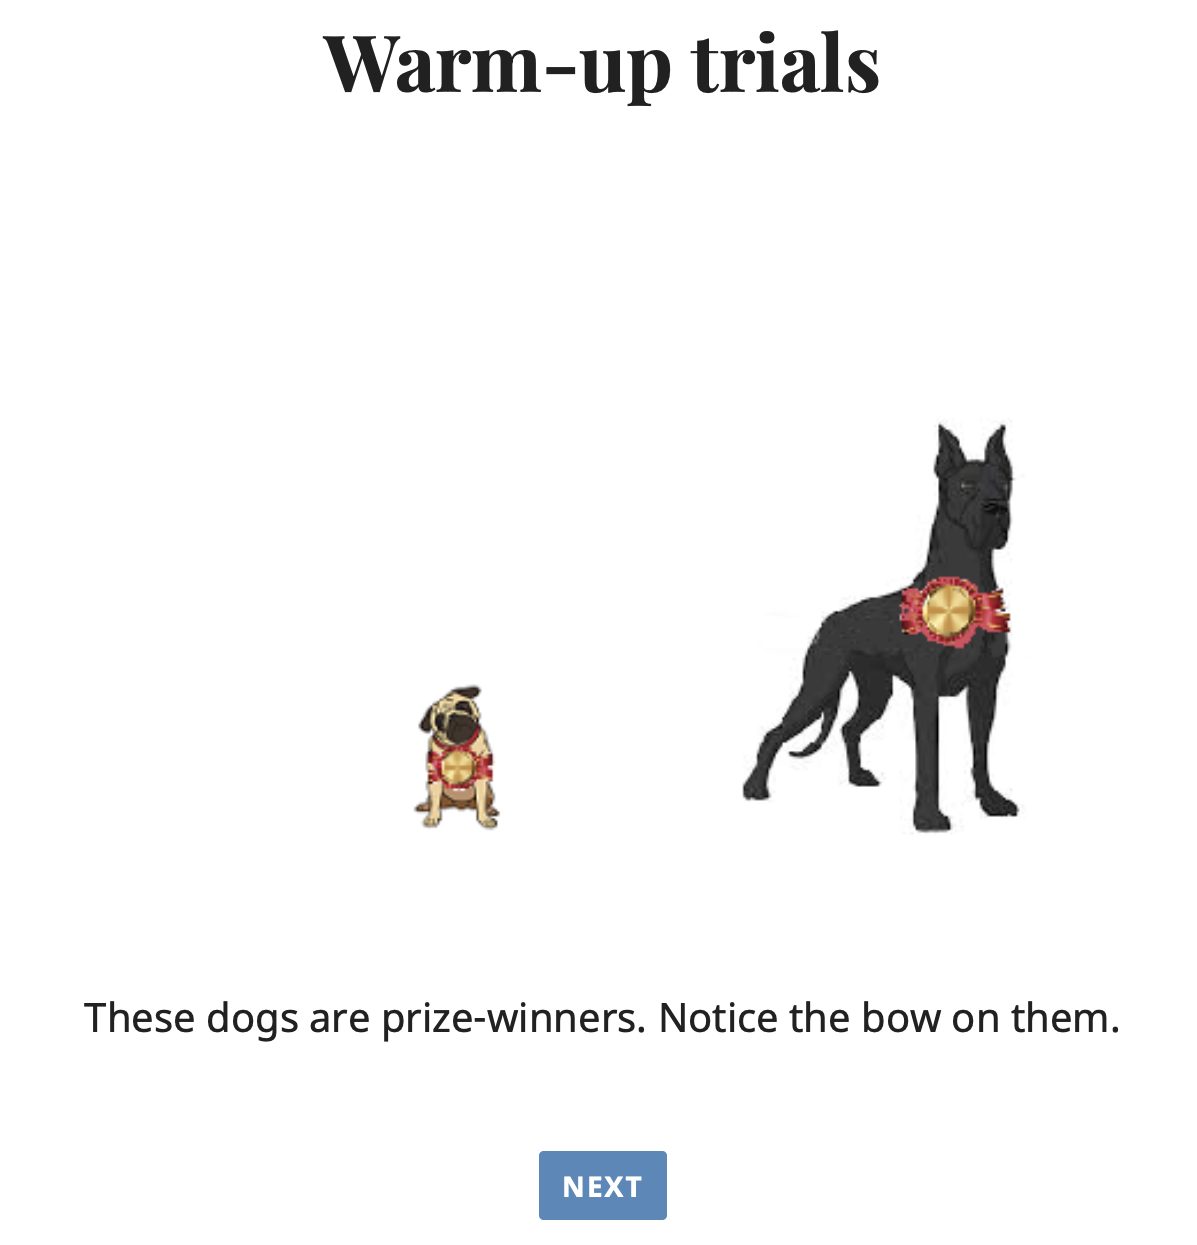
\includegraphics[width=0.6\linewidth]{direct-mod-N2-warmup.png}
	\end{center}
	\vspace{-0.3cm}
	\caption{Experiment 4 feature demonstration trial: Participants learn about additional features of the referents used on one critical main trial. For the dog-context participants learn that the pug and the Great Dane are prize-winners, indicated by bows on them.}
	\label{double-mod-N2warmup}
\end{figure*} 
The experimental set-up was similar to Experiment 3. Five different contexts were used in this experiment: there were two dog contexts, a flower, a bird and a tree context (Table \ref{stims:e4}). Four out of five contexts were randomly sampled for each participant.  Participants completed two experimental blocks, each consisting of warm-up and main trials using two of the sampled categories. In the first block, participants first completed three rounds of labeling warm-up trials. A round consisted of a demonstration trial where participants saw two subordinate members of a basic-level category used in this block and read their labels. For example, they saw pictures of a Great Dane and a pug next to each other and read “This is a Great Dane” and “This is a pug”, respectively. They could proceed after 3.5 seconds to the next trial where they had to label other instances of the same categories themselves. They also had to provide a common label for the pictures (i.e., dogs; see Fig.~\ref{warmup-production}). The order of the pictures was randomized between-participants. They were provided feedback on their labels and could proceed only after correcting their labels.  After two labeling warm-up rounds, participants completed two demonstration trials of at least 3.5 seconds each, learning about the additional features of the referents described by the second noun of the critical sentences in main trials (Table \ref{stims:e4}). For example, participants saw a picture depicting the Great Dane and the pug with prize-bows, and read: “These dogs are prize-winners. Notice the bow on them.” (Fig.~\ref{double-mod-N2warmup}). Finally, participants completed a comparison class paraphrase practice trial, identical to the one used in Experiment 3. The warm-up trials in the second experimental block were identical, but there was no paraphrase practice trial.  

\begin{figure*}[t]
	\begin{center}
		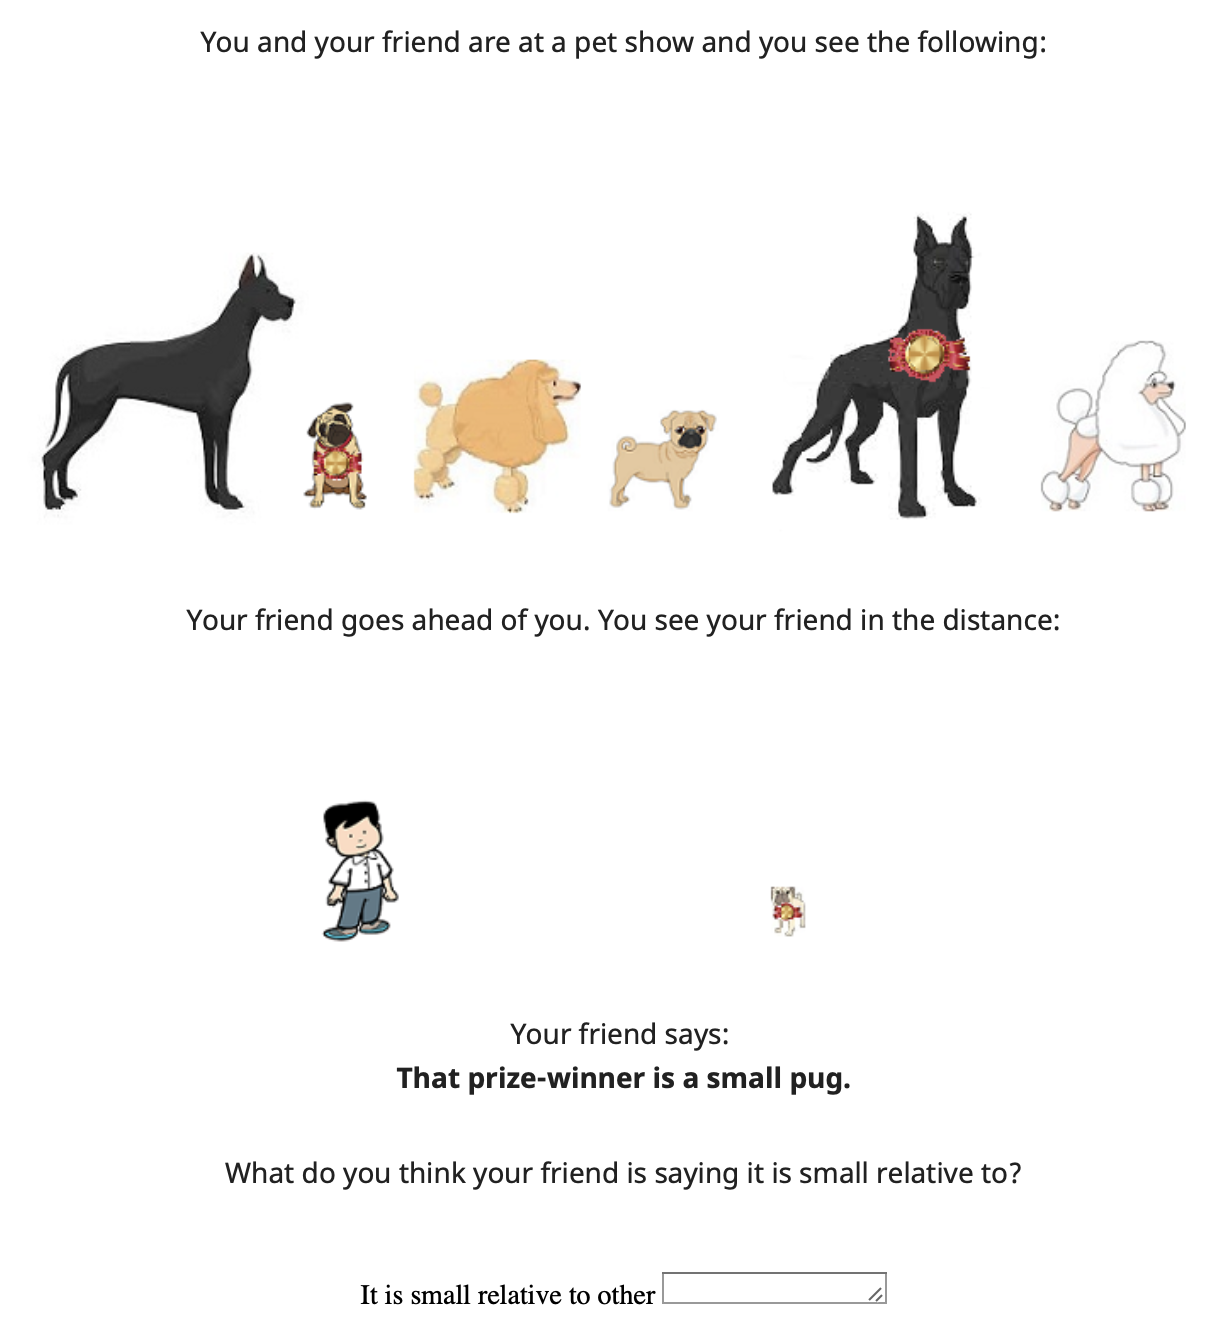
\includegraphics[width=0.6\linewidth]{double-mod-main.png}
	\end{center}
	\vspace{-0.3cm}
	\caption{Example critical main trial in Experiment 4: Participants see a dog-context and read the corresponding cover story. The small-subordinate referent is described by a predicate-noun sentence.}
	\label{double-mod-main}
\end{figure*} 
Then, participants completed four main trials - two critical and two filler trials, in randomized order, where a filler trials was always the first trial of the block. In the critical trials, a subordinate referent with an additional feature (e.g., a prize-winner bow) appeared in the corresponding context, as described above (Fig.~\ref{double-mod-main}). Participants read different context stories for each context (Table \ref{stims:e4}).  For example, for a dog context, they read “You and your friend are at a pet show and you see the following:” above the context picture. Below, they read “Your friend runs far ahead of you. You see your friend in the distance:”, followed by a depiction of the referent with the additional feature next to a person; to induce the illusion of distance, both were small relative to the context picture. Then they read “Your friend says:”, followed by the critical sentence. Finally, they were asked: “What do you think your friend is saying it is {big, small} relative to?”, introducing the paraphrase template, like in Experiment 3. For a given category, one of the possible targets appeared in this critical trial (e.g., the Great Dane). The other possible target (i.e., the pug) then appeared in a filler trial in the same block. Filler trials were identical to main trials with basic-level contexts and subordinate nouns from Experiment 3. The referent-size (i.e., large-subordinate vs. small-subordinate) was counterbalanced across syntactic conditions and trial types within-participant, resulting in 8 unique conditions. Each participant saw each condition once, resulting in eight main trials.\footnote{The experimental design described here is the final design which will be used in the main study. This design was used in the last pilot where 36 participants were recruited. The preceding pilot where 17 participants were recruited only differed from the described design in that there were no feature demonstration trials, participants did not provide common labels in the labeling warm-ups and the conditions were not counter-balanced across referent-sizes.}

%\pt{Include predictions and numerical expectations; include note about differences bw pilot 5 and 6: warm-up trials in pilot 5 had no basic-level labelling task.}

According to the reference-predication hypothesis, participants should be more likely to take the noun as signalling the comparison class when it appears in the predicate than when it appears in the subject \emph{irrespective} of modification. That is, in the critical trials where the noun is always directly modified by the adjective, a higher proportion of subordinate comparison classes is expected to be inferred in the predicate condition, compared to the subject condition. A credible positive estimate of the respective contrast would support this prediction. Further, since the filler condition replicates the condition of interest from Experiment 3, the same pattern is expected for those trials. Therefore, no difference is expected between the trial types, such that the respective regression coefficient for the trial effect is not expected to be credible.     

\subsection{Participants}
The results reported here were gathered from \rlgetvariable{myvars-direct-mod.csv}{nSubj} participants recruited in two pilot studies.\footnote{The number of participants for the main experiment was determined via a Bayesian power analysis and revealed that 300 participants were required for a power $>$ 0.85 \parencite{kruschke2014doing, powerKurz}. The main study is in progress.} \rlgetvariable{myvars-direct-mod.csv}{nExcludedTotal} participants were excluded for indicating a native language other than English, or failing either the comparison class inference practice trial or the labeling warm-up trials more than four times upon correction. The experiment took about 7 minutes and participants were compensated \$1.00.   
 
\subsection{Results}
\begin{figure*}[t]
	\begin{center}
		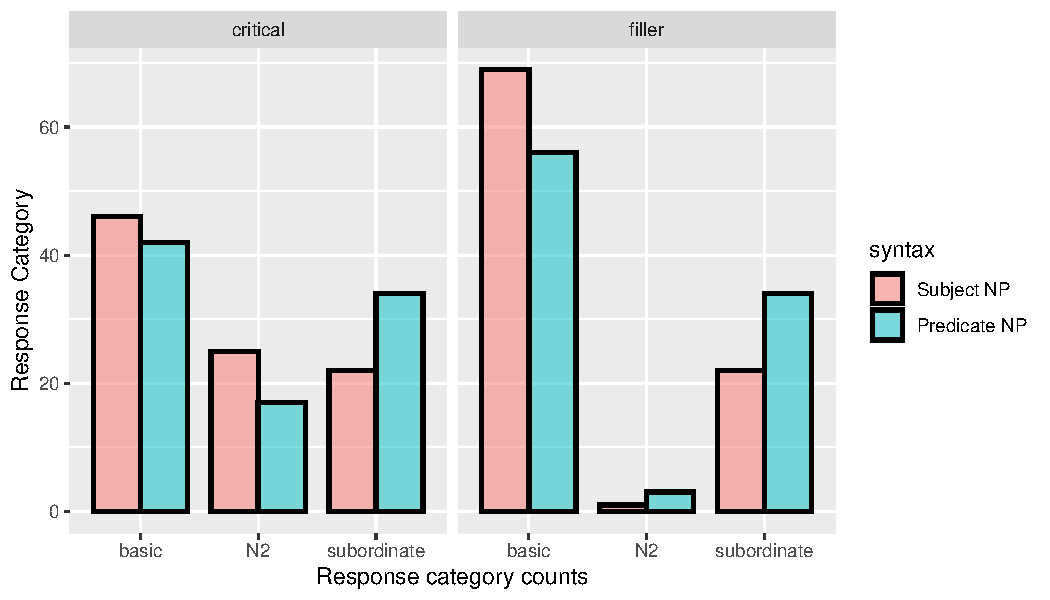
\includegraphics[width=0.8\linewidth]{double_mod_resp_counts.pdf}
	\end{center}
	\vspace{-0.3cm}
	\caption{Response categories produced in Experiment 4 pilot: Counts of different response types (basic-level target labels, subordinate target labels, N2 denoting the visual feature in critical trials; x-axis) when the subordinate noun occured in different positions (color),  by trial type (facets).}
	\label{double-mod-resp-counts}
\end{figure*}

\begin{figure*}[h]
	\begin{center}
		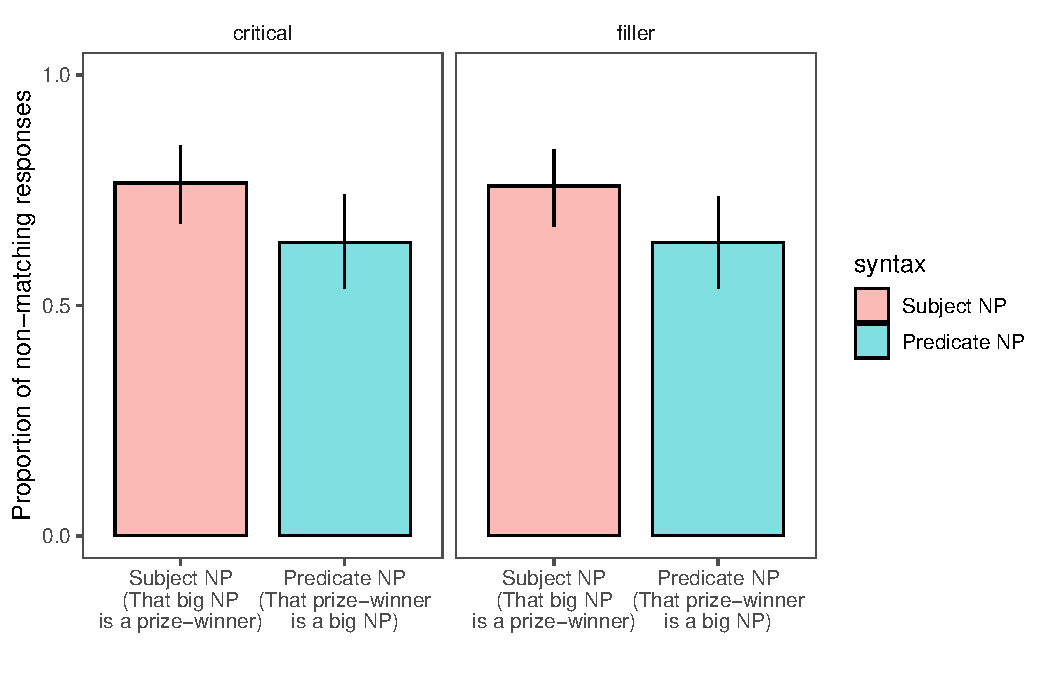
\includegraphics[width=0.7\linewidth]{double_mod.pdf}
	\end{center}
	\vspace{-0.3cm}
	\caption{Experiment 4 pilot results: Proportions of inferred comparison classes in terms of responses not matching the critical subordinate target label (e.g.,~“...big relative to other dogs/prize-winners/animals”), depending on syntactic position of the noun (x-axis) and trial-type (facets). Error-bars denote bootstrapped 95\% confidence intervals.}
	\label{double-mod-results}
\end{figure*}


Participants' responses were manually classified into responses matching the critical subordinate referent label noun (i.e. subordinate comparison classes) and non-matching responses. That is, non-matching responses included basic-level or superordinate nouns as well as the second supplementary feature-nouns (e.g., "...relative to other prize-winners"). Compound modified nouns were classified according to the head noun: for instance, responses like "prize-winning Great Danes" were classified as matching, and responses like "floral gifts" were classified as non-matching. The overall proportion of responses matching the supplementary feature-nouns was 12.4 \%, and more of these nouns were provided when this noun appeared in the predicate than in the subject position (Fig.~\ref{double-mod-resp-counts}). 
13 uncategorizable responses (3.4\%) were excluded from analysis. 
A Bayesian logistic mixed-effects regression model was used, predicting the response category from the syntactic condition (subject-N~vs.~predicate-N), the trial type (critical~vs.~filler) and their two-way interaction. By-participant and by-item random intercepts and random slope effects of both predictors and their interaction were included.\footnote{In brm-style syntax: \texttt{response\_category $\sim$ syntax*trial\_type + (1 + syntax*trial\_type | subject) + (1 + syntax*trial\_type | target)}}  
Default priors were used. The predictors were sum-coded, coding the subject-N syntax and filler trials as 1, the predicate-N syntax and critical trials as -1.\footnote{Preliminary results of this experiment from a different pilot were presented as a poster at AMLaP 2020 \parencite{TesslerEtAl2020AMLaP}. }

In line with predictions made by the reference-predication trade-off hypothesis, participants were sensitive to the syntactic position of the noun irrespectively of syntactic modification: even given directly modified nouns, in the critical trials pariticipants were more likely to infer the subordinate comaprison class when the subordinate noun phrase appeared in the predicate compared to the subject position ($\beta = \rlgetnum{expt4_contrasts.csv}{Rowname}{syntax_critical}{mean}{2} [\rlgetnum{expt4_contrasts.csv}{Rowname}{syntax_critical}{lower}{2},  \rlgetnum{expt4_contrasts.csv}{Rowname}{syntax_critical}{upper}{2}]$; Fig.~\ref{double-mod-results}, left facet). 
Furthermore, supporting the findings from Experiment 3, in the filler trials participants were also more likely to infer subordinate comparison classes from subordinate nouns in the predicate rather than in the subject position ($\beta = \rlgetnum{expt4_contrasts.csv}{Rowname}{syntax_filler}{mean}{2} [\rlgetnum{expt4_contrasts.csv}{Rowname}{syntax_filler}{lower}{3},  \rlgetnum{expt4_contrasts.csv}{Rowname}{syntax_filler}{upper}{2}]$; Fig.~\ref{double-mod-results}, right facet). Overall, participants inferred more subordinate comparison classes when the subordinate noun appeared in the predicate than when it appeared in the subject, across trial types ($\beta = \rlgetnum{expt4_contrasts.csv}{Rowname}{syntax_subj_v_pred}{mean}{2} [\rlgetnum{expt4_contrasts.csv}{Rowname}{syntax_subj_v_pred}{lower}{2},  \rlgetnum{expt4_contrasts.csv}{Rowname}{syntax_subj_v_pred}{upper}{2}]$). Consistent with the prediction that syntactic modification which was varied between trial types should not play a role for comparison class inference, no credible effects of trial type or difference in syntax-effects on different trial-types were observed (trial effect: $\beta = \rlgetnum{expt4_contrasts.csv}{Rowname}{trial_filler_v_critical}{mean}{2} [\rlgetnum{expt4_contrasts.csv}{Rowname}{trial_filler_v_critical}{lower}{2},  \rlgetnum{expt4_contrasts.csv}{Rowname}{trial_filler_v_critical}{upper}{2}]$, Fig.~\ref{double-mod-results}, left~vs.~right facet; trial $\times$ syntax interaction estimate: $\beta = \rlgetnum{expt4_contrasts.csv}{Rowname}{b_syntax_sum1:trial_sum1}{mean}{2} [\rlgetnum{expt4_contrasts.csv}{Rowname}{b_syntax_sum1:trial_sum1}{lower}{2},  \rlgetnum{expt4_contrasts.csv}{Rowname}{b_syntax_sum1:trial_sum1}{upper}{2}]$, Fig.~\ref{double-mod-results}, left~vs.~right bar in left~vs.~right facet).  

This experiment provided evidence that participants are able to flexibly reason about informational goals the nouns which combined with the adjective are intended for, above and beyond syntactic modification. These results show that the primary driver behind the cue-strength of the noun towards the comparison class is indeed the informational goal that the noun accomplishes, and not the modification of the noun by the adjective.  Therefore, it can be ruled out that nouns appearing in the predicate position of the utterance provided a stronger cue towards the comaprison class than nouns in the subject just due to direct modification by the adjective (cf. experiments 1-3). 

Together with Experiment 3, these results show that listeners flexibly adjust comparison classes by reasoning about informational goals and sentence structure, integrated with perceptual cues and their general world knowledge.   
   
